\documentclass{beamer}

\usepackage[utf8]{inputenc}
%\usepackage[scaled]{uarial} % not available in Linux
\renewcommand{\rmdefault}{phv} % Arial

\renewcommand{\sfdefault}{phv} % Arial
\renewcommand*\familydefault{\sfdefault} %% Only if the base font of the document is to be sans serif

\usepackage[T1]{fontenc}
\usepackage{classico}
\usepackage{siunitx}
\sisetup{
separate-uncertainty,
separate-uncertainty-units = bracket}

\usepackage{physics}
\usepackage{bm}
  \SetSymbolFont{largesymbols}{bold}{OMX}{txex}{b}{n} % for big bold parethesis

\title{Classificazione dei bosoni elettrodeboli con una rete neurale al Large Hadron Collider} 
\subtitle{6 Novembre 2024}
\date{6 Novembre 2024}
\author{Jacopo Lancione}

\usetheme{UNITO}
    %\setbeamercovered{invisible} %default
  \setbeamercovered{transparent} % Items to be uncovered already visible, but almost transparent
    
\begin{document}
\begin{frame}
    \titlepage
\end{frame}

\begin{frame}{Sommario}
    \tableofcontents
\end{frame}


\section{Introduzione}
\begin{frame}
  \centering
  \Huge\bfseries
  Introduzione
\end{frame}

\subsection{LHC}
\begin{frame}{Large Hadron Collider - CMS}
% \begin{figure}
%   \centering
%   \begin{tikzpicture}
%     \node [inner sep=0pt, minimum width=.5cm, minimum height=.5cm] (cern) at ($(-\the\paperwidth/2,-\the\paperheight/2) + (-3.2,-.3)$) {
%       
\includegraphics[width=.1\linewidth]{./Images/cern_logo.pdf}
%     };
%     \node [inner sep=0pt, minimum width=.5cm, minimum height=.5cm] (cms_logo) at ($(cern) + (1.5,0)$){
%       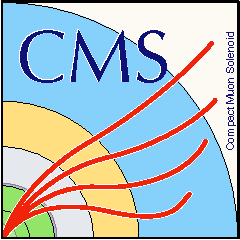
\includegraphics[width=.1\linewidth]{./Images/cms_logo.pdf}
%     };
%     \node [draw, line width=.1cm, inner sep=0pt, text width=9cm, minimum height=6cm] (cms) at (-1.64,-2.5) {
%       \includegraphics[width=\textwidth]{./Images/cms_cutaway.pdf}
%     };
%     \node [draw, line width=.1cm, inner sep=0pt, text width=5cm] (text) at ($(cern) + (1.0,\the\paperheight/3)$) {
%       Il più grande acceleratore di particelle del mondo di cui il Compact Muon Solenoid (CMS) è uno dei quattro rivelatori principali. 
%     };
%   \end{tikzpicture}
  \begin{columns}
    \column{.20\linewidth}
      \begin{figure}
        \centering
        
\includegraphics[width=.5\textwidth]{./Images/cern_logo.pdf}\\
        \vspace{1ex}
        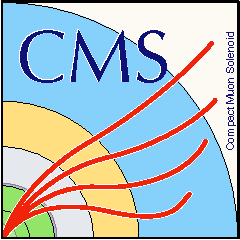
\includegraphics[width=.5\textwidth]{./Images/cms_logo.pdf}
      \end{figure}
    \column{.80\linewidth}
      \vspace{-1ex}
      \begin{figure}
        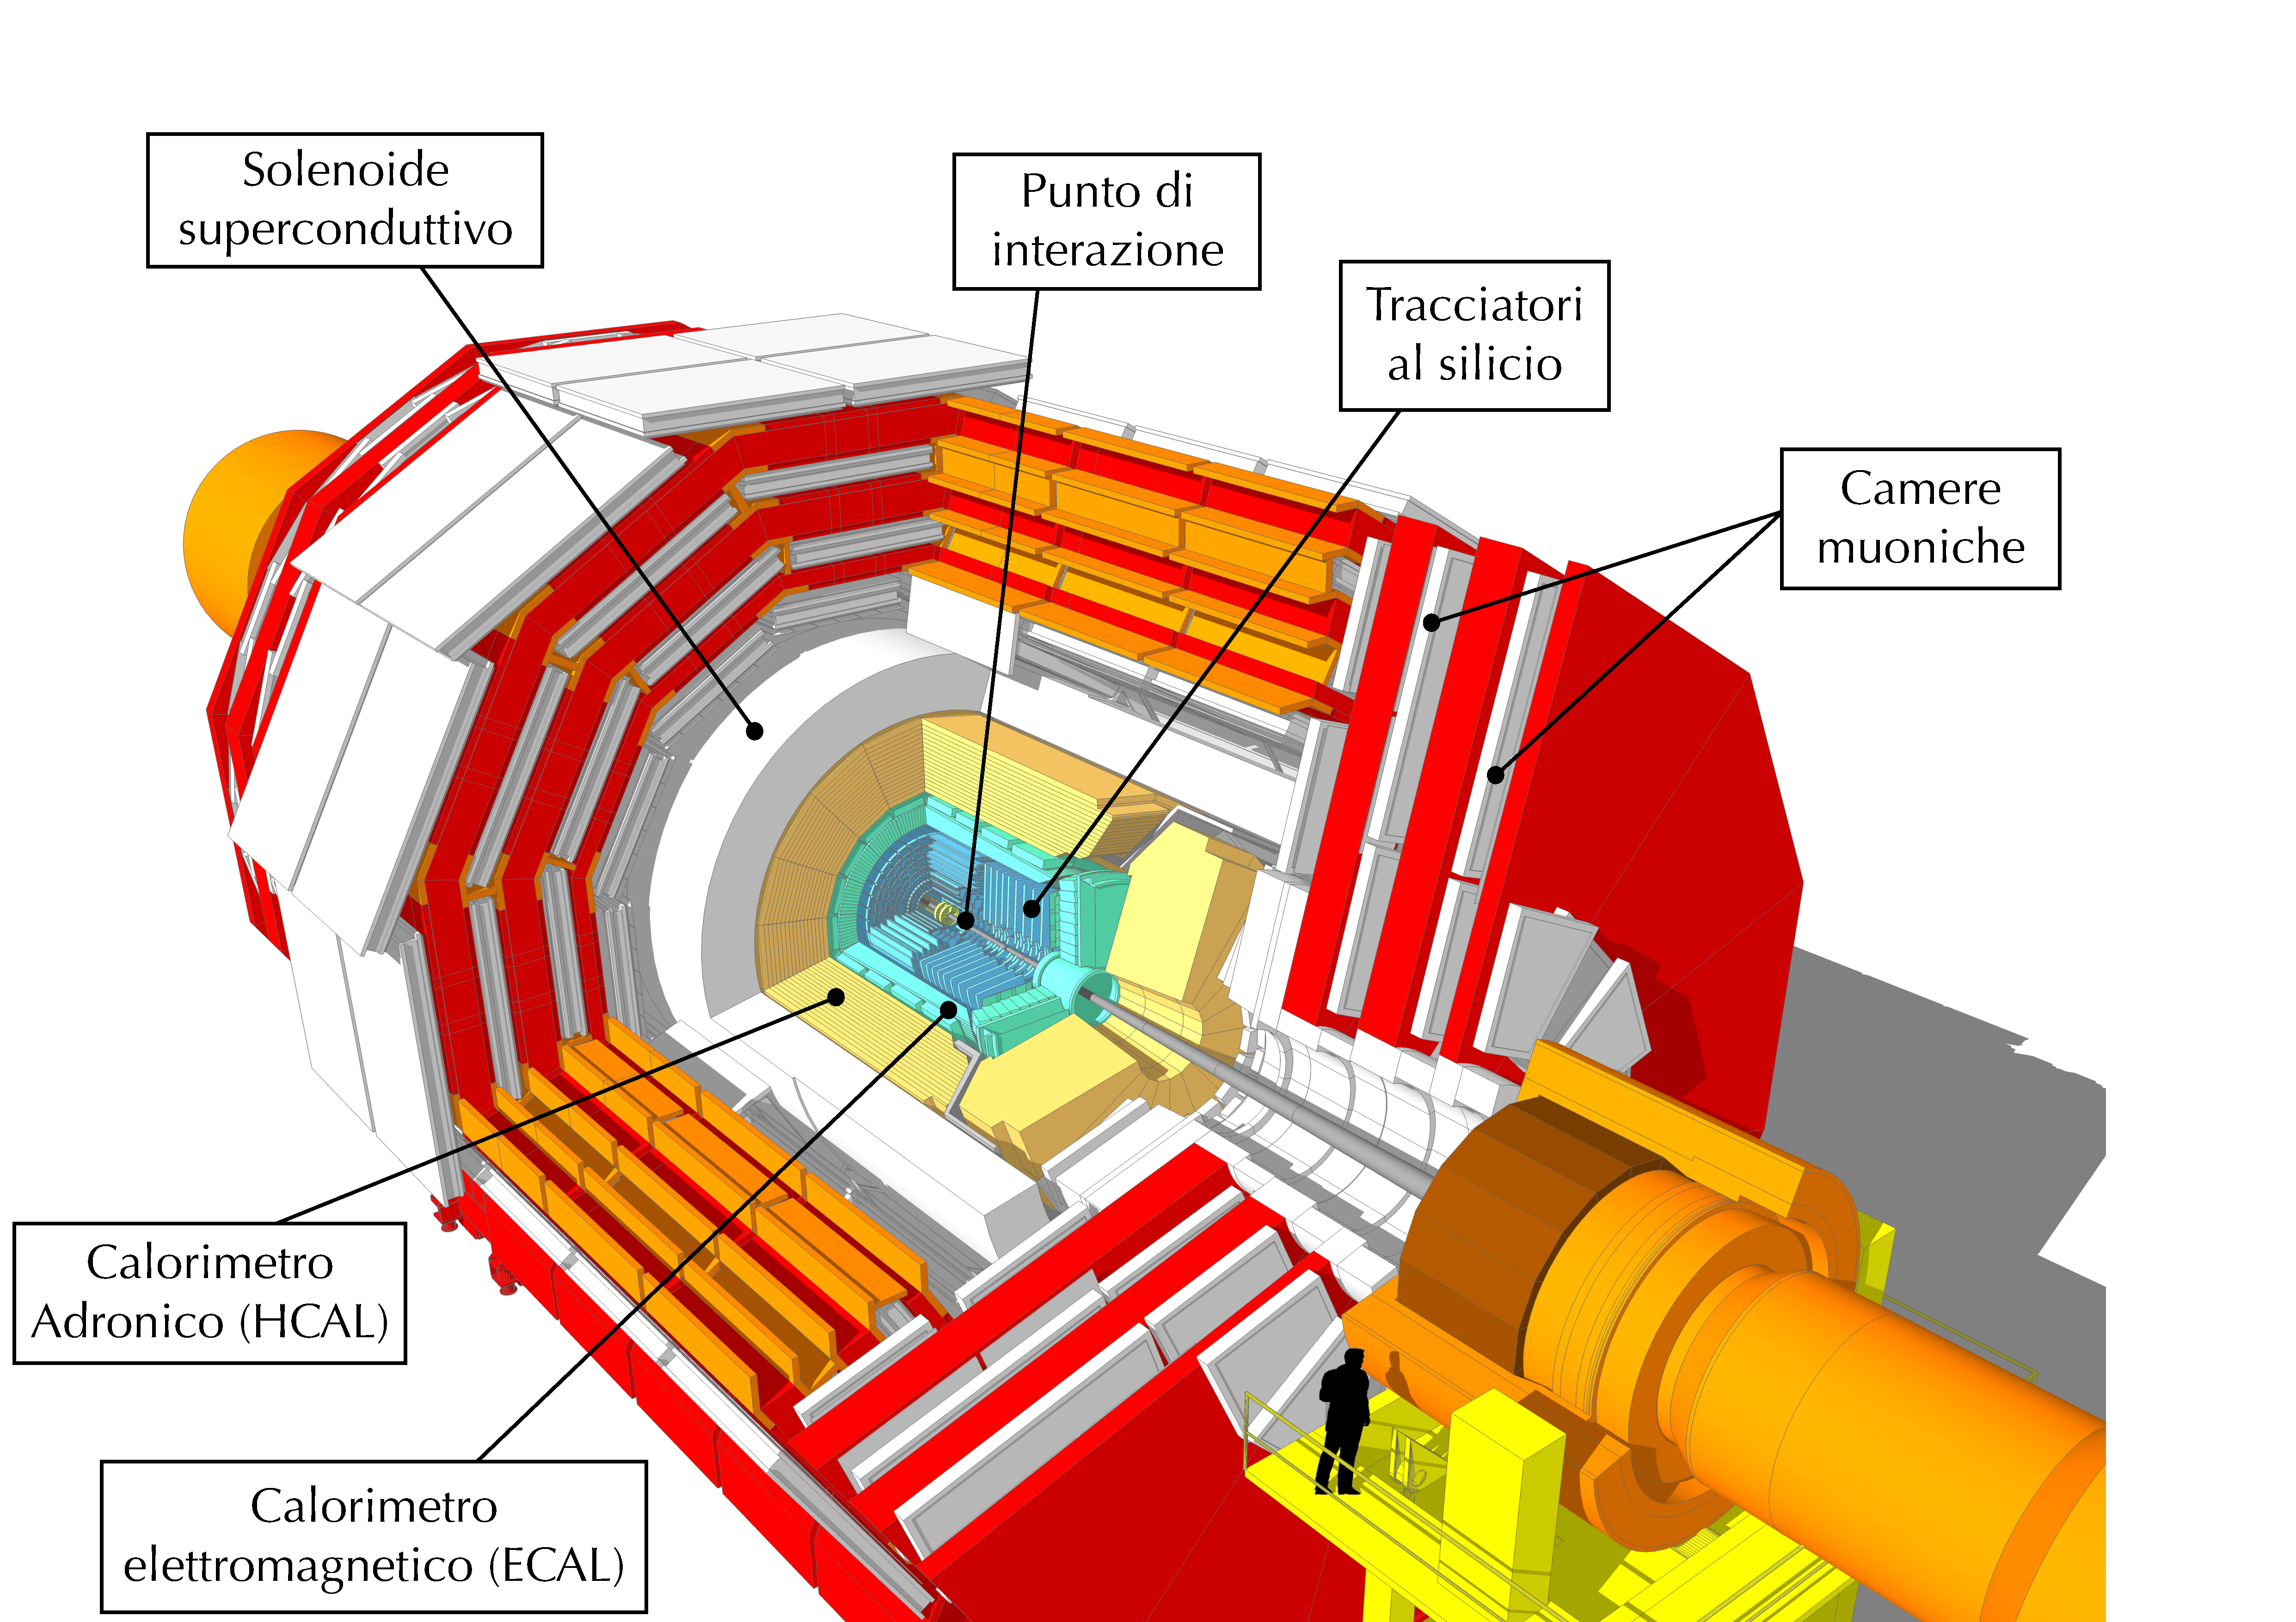
\includegraphics[width=\textwidth]{./Images/cms_cutaway-flat.pdf}
      \end{figure}
      \begin{flushright}
        \vspace{-3.3ex}
        \scalebox{.4}{\color{unitograyA!65}
          Image adapted from https://cds.cern.ch/record/2665537
        }
      \end{flushright}
    \end{columns}
% L'anello di accelerazione + grande del mondo, parliamo del CMS da cui arrivano i miei dati, in cui si producono particelle in abbondanza,
% Del CMS mi interessa giusto introdurre il fatto che ci siano dei calorimetri perché alcuni loro parametri sono tra le features (differenze tra i calorimetri)
%
% Si produce un enorme mole di dati e per trattarli si utilizzano anche tecniche di machine learning (e così passo alla prox slide)
\end{frame}

\subsection{Machine Learning}
\begin{frame}{Machine Learning: uno sguardo d'insieme}
  \vspace*{-3ex}
  \begin{figure}
    \centering
    \resizebox{\linewidth}{!}{
      \begin{tikzpicture}[mindmap, outer sep=0pt,
        level 1 concept/.append style={level distance=148},
        level 2 concept/.append style={level distance=120},
        text=white,
        decoration={start radius=1cm, end radius=.5cm,amplitude=2mm,angle=30}]%,
%
        \only<-2>{
          \node [circle, minimum width=3.2cm, fill=unitocolor] (ml) at (0,0) {\huge\color{white}Machine\\[.5ex] Learning}
            child [grow=-10]
              {node [circle, minimum width=3.3cm, fill=unitograyA!60] (unsup) {\Large \!\!\!\!\!\!Unsupervised Learning}
                child [grow=-40]{ node[circle, minimum width=2.5cm, fill=unitocolor](clust)  {\normalsize Clustering}}
                child [grow=-85]{ node[circle, minimum width=2.5cm, fill=unitocolor](reduct) {\normalsize Riduzione dimensionale}}
              }
            child [grow=190] 
              {node [circle, minimum width=3.3cm, fill=unitograyA!60] (sup) {\Large Supervised Learning}
                child [grow=220]{ node[circle, minimum width=2.5cm, fill=unitocolor](classif) {\normalsize Classifi\-cazione}}
                child [grow=-95]{ node[circle, minimum width=2.5cm, fill=unitocolor](regr)    {\normalsize \!\!\!Regressione}}
          };
        }
        \only<3>{
          \node [circle, minimum width=3.2cm, fill=unitocolor] (ml) at (0,0) {\huge\color{white}Machine\\[.5ex] Learning}
            child [grow=-10]
              {node [circle, minimum width=3.3cm, fill=unitograyA!60] (unsup) {\Large \!\!\!\!\!\!Unsupervised Learning}
                child [grow=-40]{ node[circle, minimum width=2.5cm, fill=unitocolor](clust)  {\normalsize Clustering}}
                child [grow=-85]{ node[circle, minimum width=2.5cm, fill=unitocolor](reduct) {\normalsize Riduzione dimensionale}}
              }
            child [grow=190] 
              {node [circle, minimum width=3.3cm, fill=unitograyA!60] (sup) {\Large Supervised Learning}
                child [grow=220]{ node[circle, minimum width=2.5cm, fill=faircolor](classif) {\normalsize\color{black} Classifi\-cazione}}
                child [grow=-95]{ node[circle, minimum width=2.5cm, fill=unitocolor](regr)    {\normalsize \!\!\!Regressione}}
            };
          }

        \path (ml) to[circle connection bar switch color=from (unitocolor) to (unitograyA!60)] (unsup);
        \path (ml) to[circle connection bar switch color=from (unitocolor) to (unitograyA!60)] (sup);
        \path (unsup) to[circle connection bar switch color=from (unitograyA!60) to (unitocolor)] (clust);
        \path (unsup) to[circle connection bar switch color=from (unitograyA!60) to (unitocolor)] (reduct);
        \only<-2>{
          \path (sup) to[circle connection bar switch color=from (unitograyA!60) to (unitocolor)] (classif);
        }
        \only<3>{
          \path (sup) to[circle connection bar switch color=from (unitograyA!60) to (faircolor)] (classif);
        }
        \path (sup) to[circle connection bar switch color=from (unitograyA!60) to (unitocolor)] (regr);

        \node [inner sep=0pt, text width=6.5cm, minimum height=4.5cm] (nobel) at ($(ml) - (0,5.5)$) {
          \only<2->{
            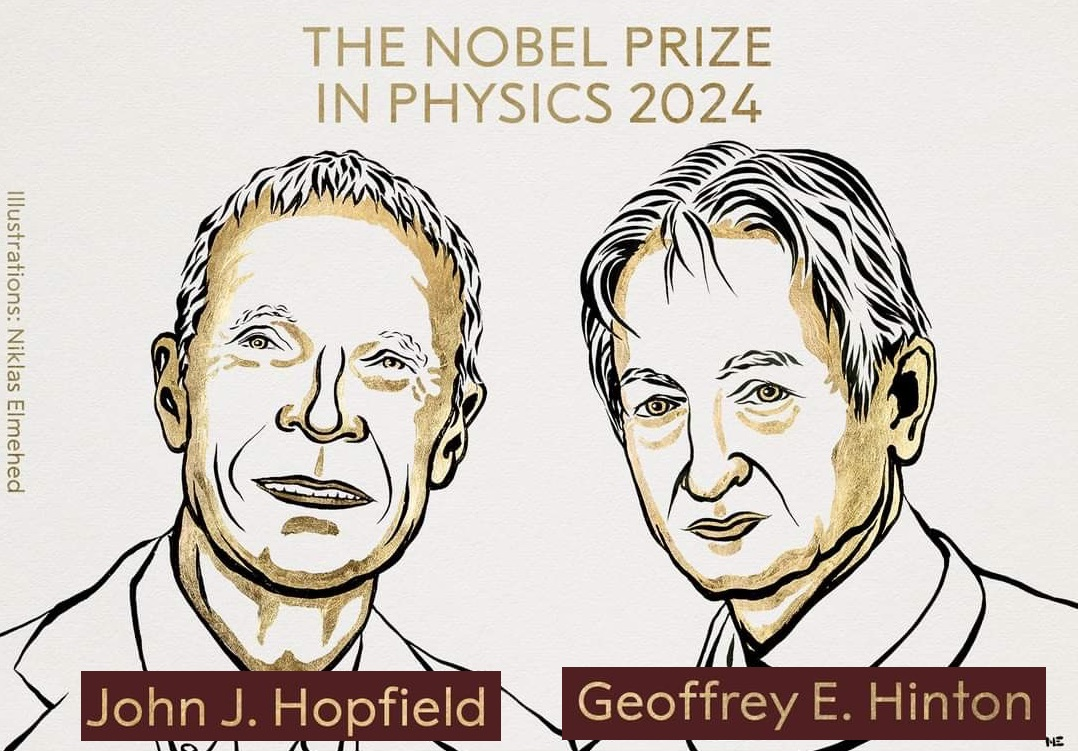
\includegraphics[width=\textwidth]{./Images/nobel_prize.jpeg}
          }
        };
      \end{tikzpicture}
    }
  \end{figure}
%
% {\scriptsize
%   In questa slide devo far passare il concetto di labeled e unlabeled data (posso anche metterle come item)
%   Supervised eccelle nla pattern recognition, che si tratti di immagini testi o (+ vicino alla fisica) trovare mapping che siano continui o meno (nel mio caso nn lo è)
%   Qua dicendo che il mio progetto ruota attorno ad un problema di classificazione passo alla prox slide
% }
\end{frame}

\begin{frame}{Il Progetto di tesi}
% {\scriptsize
%   Che sia chiaro dove si colloca il mio progetto:
%   affrontare un problema di classificazione binaria (logistic regression), nell'ambito della Fisica delle alte energie
%
%   Immagine classica del modello std e 1 di 1 rete neurale giusto per dire rapidamente il Cosa e il Come
%
%   il mio obiettivo: allenare 1 rete che distingua al meglio tra i 2 canali di decadimento
% }
  \vspace*{-3.5ex}
  \begin{center}
    \Large
    Classificare
  \end{center}
  \vspace*{-1.5ex}
  \begin{columns}[T]
    \column{.40\linewidth}
      \begin{block}{}
        \centering%
        Bosoni elettrodeboli
      \end{block}
      \begin{figure}
        \centering
        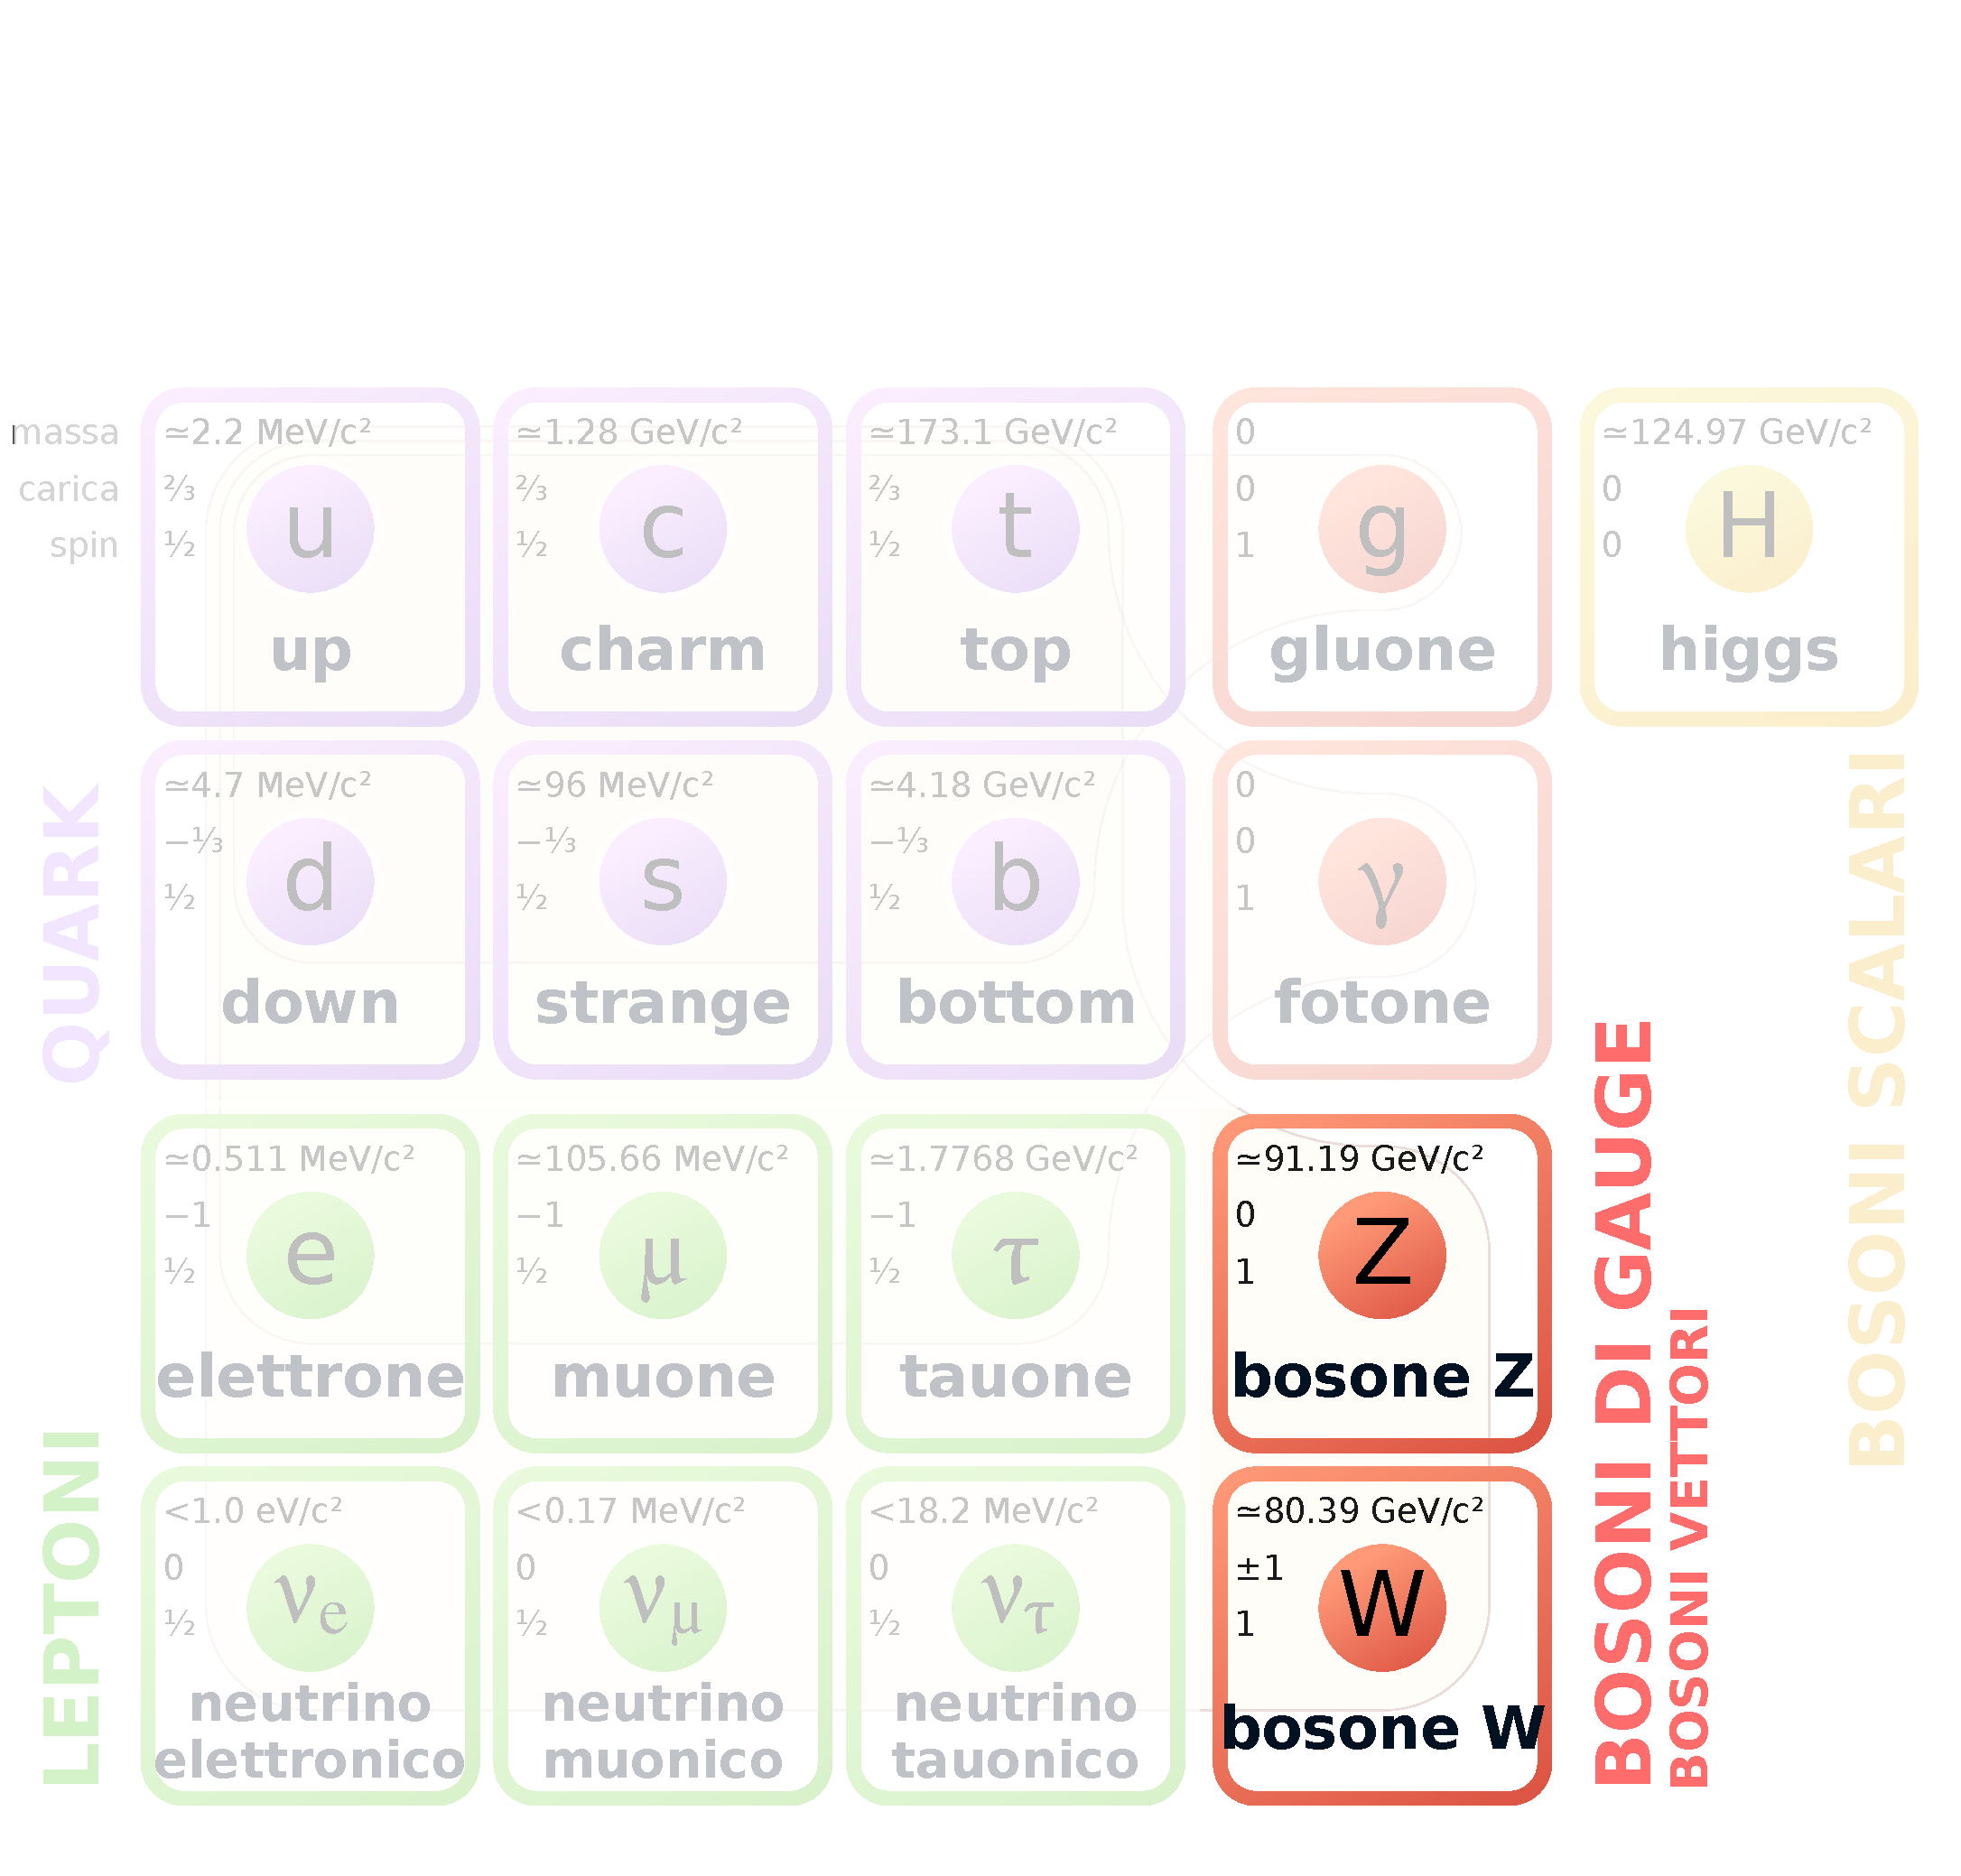
\includegraphics[width=\textwidth]{./Images/sm_overview-flat.pdf}
      \end{figure}
      \begin{flushleft}
        \vspace{-3ex}
        \scalebox{.4}{\color{unitograyA!65}
          Adapted from: https://it.wikipedia.org/wiki/Modello\_standard
        }
      \end{flushleft}
    \column{.11\linewidth}
      {
        \setbeamercolor{block body}{bg=white, fg=black}
        \begin{block}{}
          \centering\small
          con una
        \end{block}
      }
    \column{.35\linewidth}
      \begin{block}{}
        \centering
        Rete neurale
      \end{block}
      \parbox[t][][c]{\textwidth}{
        \vspace*{3ex}
        \centering
        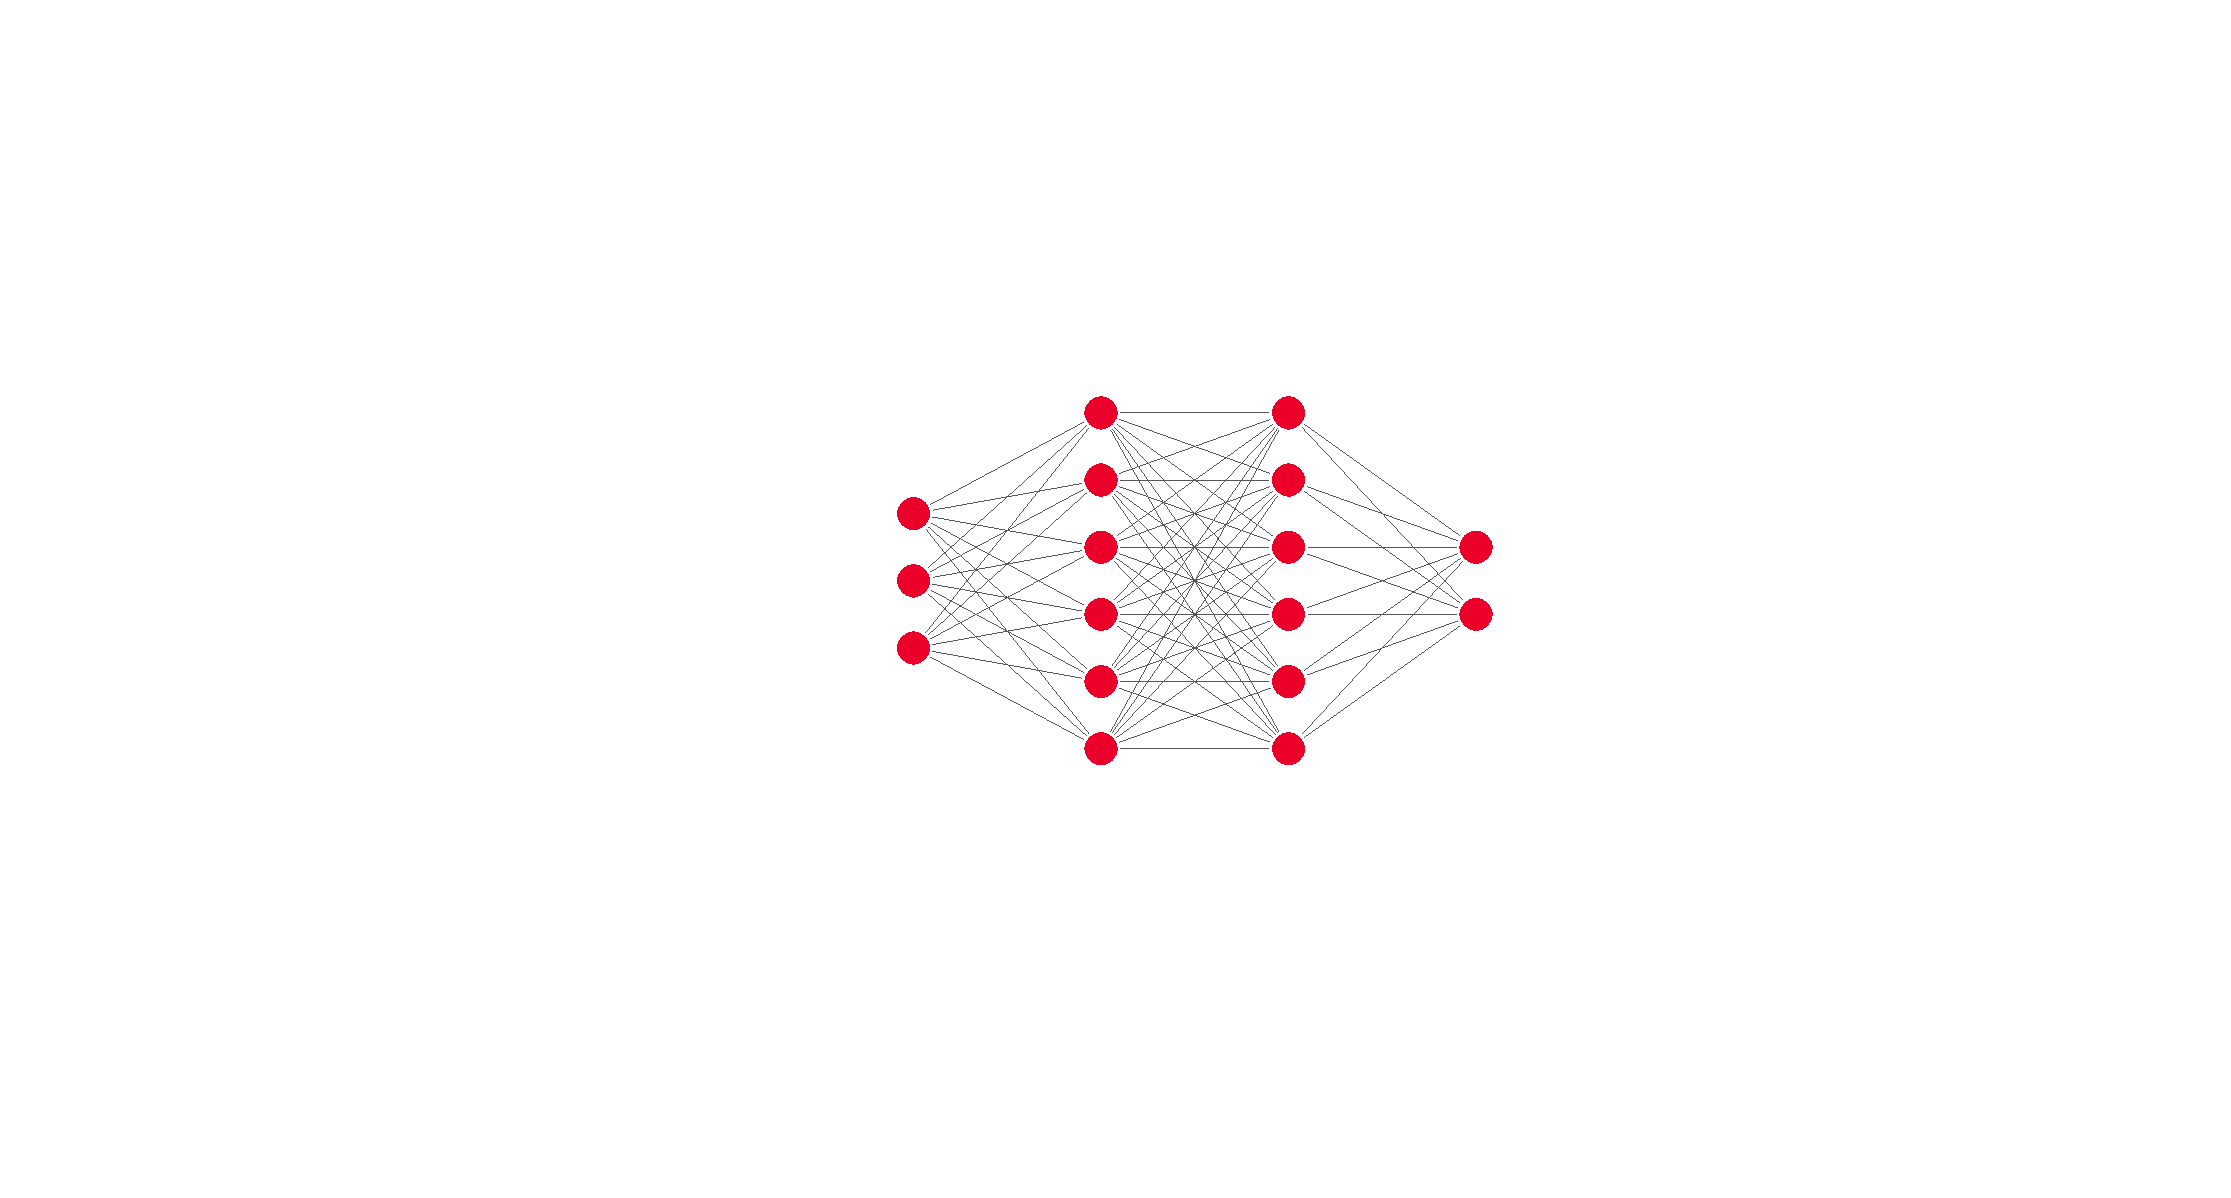
\includegraphics[width=.9\textwidth]{./Images/nn_diagram.pdf}
      }
  \end{columns}
\end{frame}

\section{Dataset}
\begin{frame}
  \centering
  \Huge\bfseries
  Il Dataset
\end{frame}

\subsection{Produzione dei bosoni}
\begin{frame}{$Z$ e $W$ all'LHC\\ Il processo Drell-Yan e il decadimento}
  \begin{columns}[T]
    \column{.43\linewidth}
      \centering
      \vspace*{1ex}
      \scalebox{1.5}{
        $p\,p \to Z \to \ell\,\overline{\ell}$%
      }%
      \vspace*{2ex}
      \begin{block}{}
        \centering
        \SI{91.188(2)}{\giga\electronvolt\per c^2}
        \vspace*{.3ex}
      \end{block}
      \vspace*{2ex}
      \begin{tikzpicture}
%         \draw [help lines] (-2,-2) grid (2,2);
        \node [line width=.1cm, text width=3.5cm] (feyn) at (0,0) {
          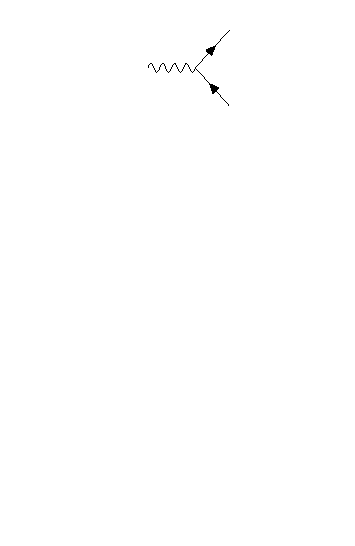
\includegraphics[width=\textwidth]{./Images/feynman_canva-flat.pdf}
        };
        \node [line width=.1cm, text width=.2cm] (Z) at (-.5,.5) {
          \centering%
          $Z$
        };
        \node [anchor=west, line width=.1cm, text width=1.5cm] (e) at (1.3,1) {
          \centering%
          $e^{-}$, $\mu^{-}$
        };
        \node [anchor=west, line width=.1cm, text width=1.5cm] (nu) at (1.3,-1) {
          \centering%
          $e^{+}$, $\mu^{+}$
        };
      \end{tikzpicture}
    \column{.003ex}
    \column{.43\linewidth}
      \centering
      \vspace*{1ex}
      \scalebox{1.5}{
        $p\,p \to W \to \ell\,\overline{\nu}$, $\nu\, \overline{\ell}$%
      }%
      \vspace*{2ex}
      \begin{block}{}
        \centering
        \SI{80.369(13)}{\giga\electronvolt\per c^2}
        \vspace*{.3ex}
      \end{block}
      \vspace*{2ex}
      \begin{tikzpicture}
%         \draw [help lines] (-2,-2) grid (2,2);
        \node [line width=.1cm, text width=3.5cm] (feyn) at (0,0) {
          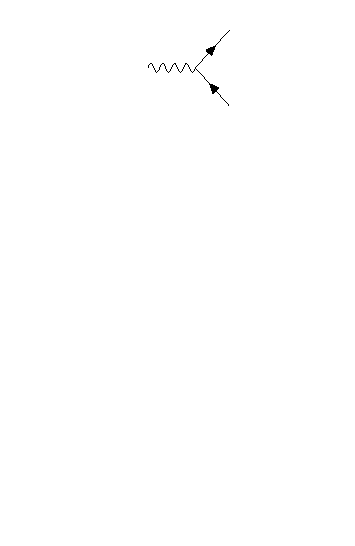
\includegraphics[width=\textwidth]{./Images/feynman_canva-flat.pdf}
        };
        \node [line width=.1cm, text width=.2cm] (W) at (-.5,.5) {
          \centering%
          $W^{-}$
        };
        \node [anchor=west, line width=.1cm, text width=1.5cm] (e) at (1.3,1) {
          \centering%
          $e^{-}$, $\mu^{-}$
        };
        \node [anchor=west, line width=.1cm, text width=1.5cm] (nu) at (1.3,-1) {
          \centering%
          $\overline{\nu}_e$, $\overline{\nu}_{\mu}$
        };
      \end{tikzpicture}
  \end{columns}

% Diagrammi di Feynman dei decadimenti, anche uno con la produzione? ie drell yan
\end{frame}

\begin{frame}{La struttura del dataset}
%  Diamo subito qlche dettaglio in $+$ sul dataset
  \begin{columns}[T]
    \column{.40\linewidth}
      \vspace*{4ex}
 %    Eventi dalla Run 1 dell'LHC
      \begin{block}{}
        \centering
        Energia nel centro di massa\linebreak
        \SI{7}{\tera\electronvolt}
        \vspace*{.3ex}
      \end{block}
      \vspace*{1ex}
    % pké risale a prima dl'upgrade che lo ha portato agli odierni 13Tev nel cm
      \begin{itemize}
        \item Run 
        \item Event
        \item Parametri dei leptoni ($Q$, $p_t$, $\eta$, $\phi$)
        \item Parametri del detector
        % gli iso, dove è stato trovato il leptone (barrel o endcap), ma cmq NN sono uniformi tra i dataset qndi ciccia :)
      \end{itemize}

    \column{.52\linewidth}
      \vspace*{4ex}
      \begin{figure}
        \centering
        \includegraphics[width=\textwidth]{./Images/cms_event.png}
      \end{figure}
  \begin{flushright}
    \vspace{-3ex}
    \scalebox{.4}{\color{unitograyA!65}
      Image from: https://cds.cern.ch/record/2909335?ln=en
    }
  \end{flushright}
  \vspace*{.7ex}
  \begin{center}
    \scriptsize
    Datasets derived from the Run2011A:\\
    https://opendata.cern.ch/record/545
  \end{center}
  \vspace*{1.5ex}
  \end{columns}
\end{frame}

\subsection{Preprocessing}
\begin{frame}{Preprocessing}
  \centering
  \vspace*{1.2ex}
  Trattamento degli outliers \,\,$\color{unitocolor}\to$\,\, Correlazioni \,\,$\color{unitocolor}\to$\,\, Normalizzazione
% \vspace*{.7ex}
  \begin{columns}[T]
    \column{.50\linewidth}
      \centering
      \begin{pgfpicture}{-1ex}{0ex}{1ex}{2ex}
        \color{unitocolor}
        \pgfpathcircle{\pgfpoint{0pt}{.5ex}}{0.4ex}
        \pgfusepath{fill}
      \end{pgfpicture} {\footnotesize $Z\to \mu^{+}\,\mu^{-}$}
      \quad
      \begin{pgfpicture}{-1ex}{0ex}{1ex}{2ex}
        \color{unitograyA}
        \pgfpathcircle{\pgfpoint{0pt}{.5ex}}{0.4ex}
        \pgfusepath{fill}
      \end{pgfpicture} {\footnotesize $Z\to e^{+}\, e^{-}$}
    \column{.50\linewidth}
      \centering
      \begin{pgfpicture}{-1ex}{0ex}{1ex}{2ex}
        \color{unitocolor}
        \pgfpathcircle{\pgfpoint{0pt}{.5ex}}{0.4ex}
        \pgfusepath{fill}
      \end{pgfpicture} {\footnotesize $W\to e\, \nu_e$}
      \quad
      \begin{pgfpicture}{-1ex}{0ex}{1ex}{2ex}
        \color{unitograyA}
        \pgfpathcircle{\pgfpoint{0pt}{.5ex}}{0.4ex}
        \pgfusepath{fill}
      \end{pgfpicture} {\footnotesize $W\to \mu\, \nu_{\mu}$}
  \end{columns}
  \begin{columns}[b]
    \column{.50\linewidth}
      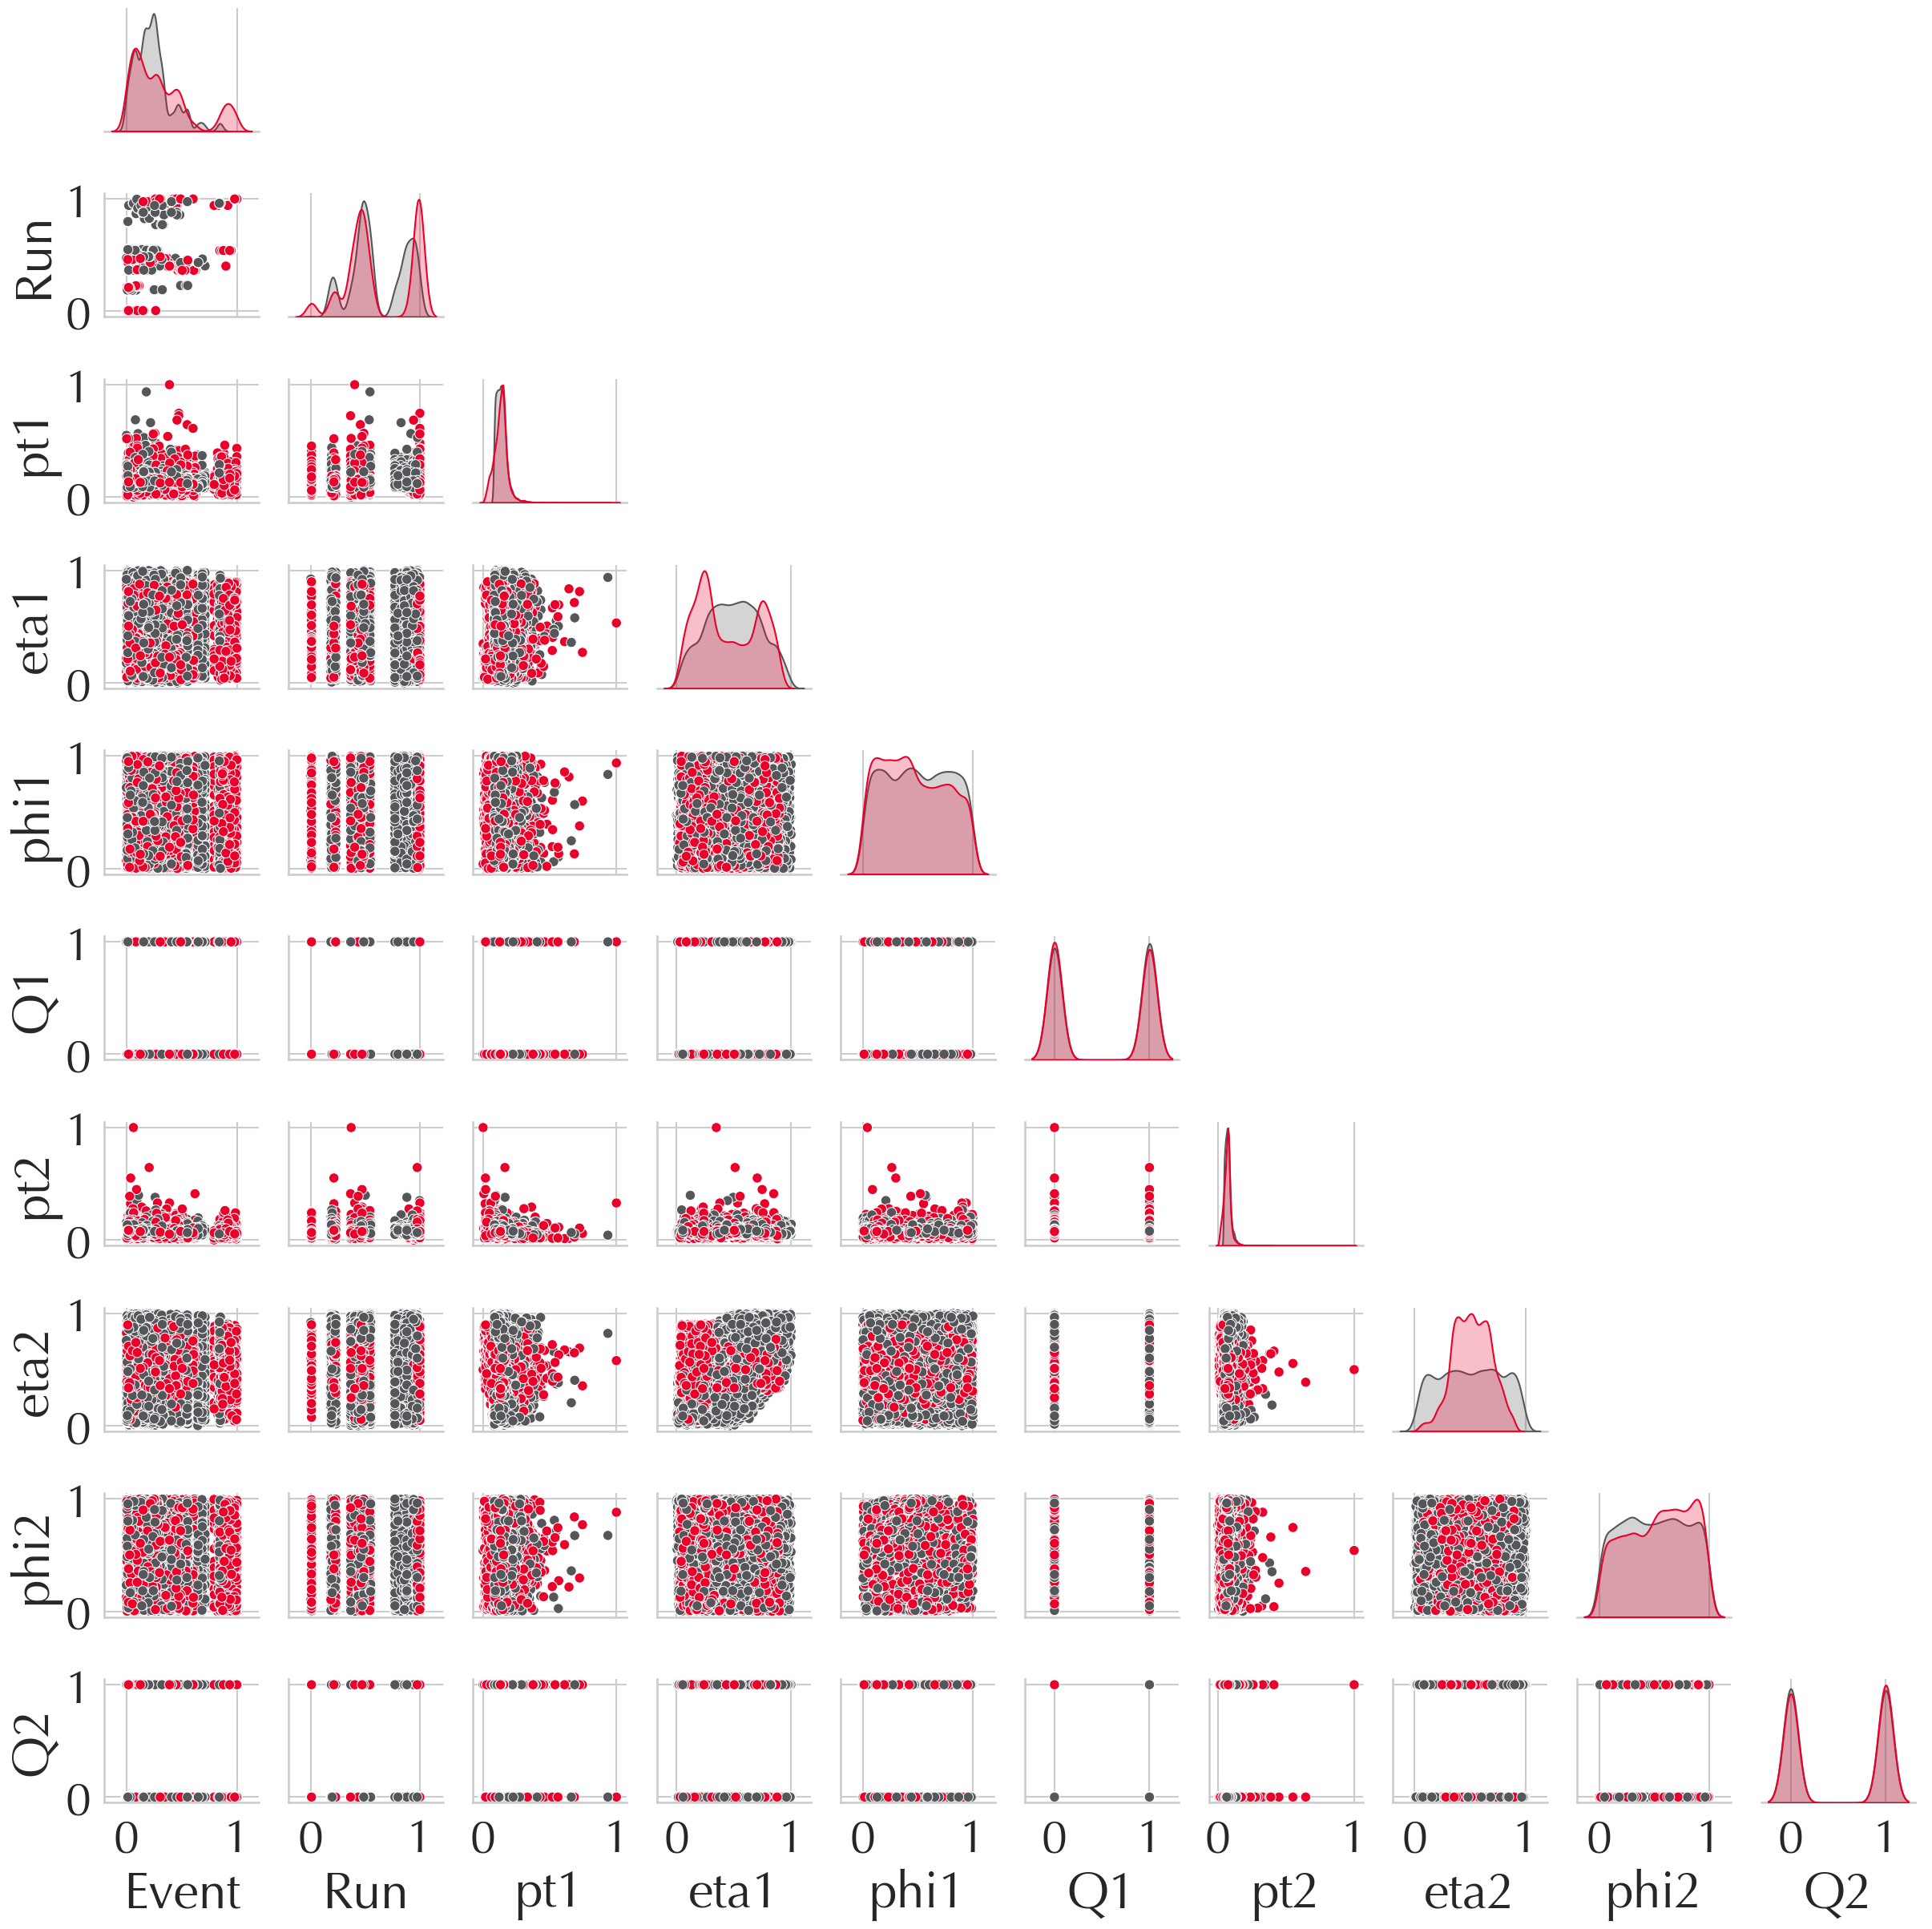
\includegraphics[width=\linewidth]{./Images/Zpairplot_scaled.png}
    \column{.50\linewidth}
      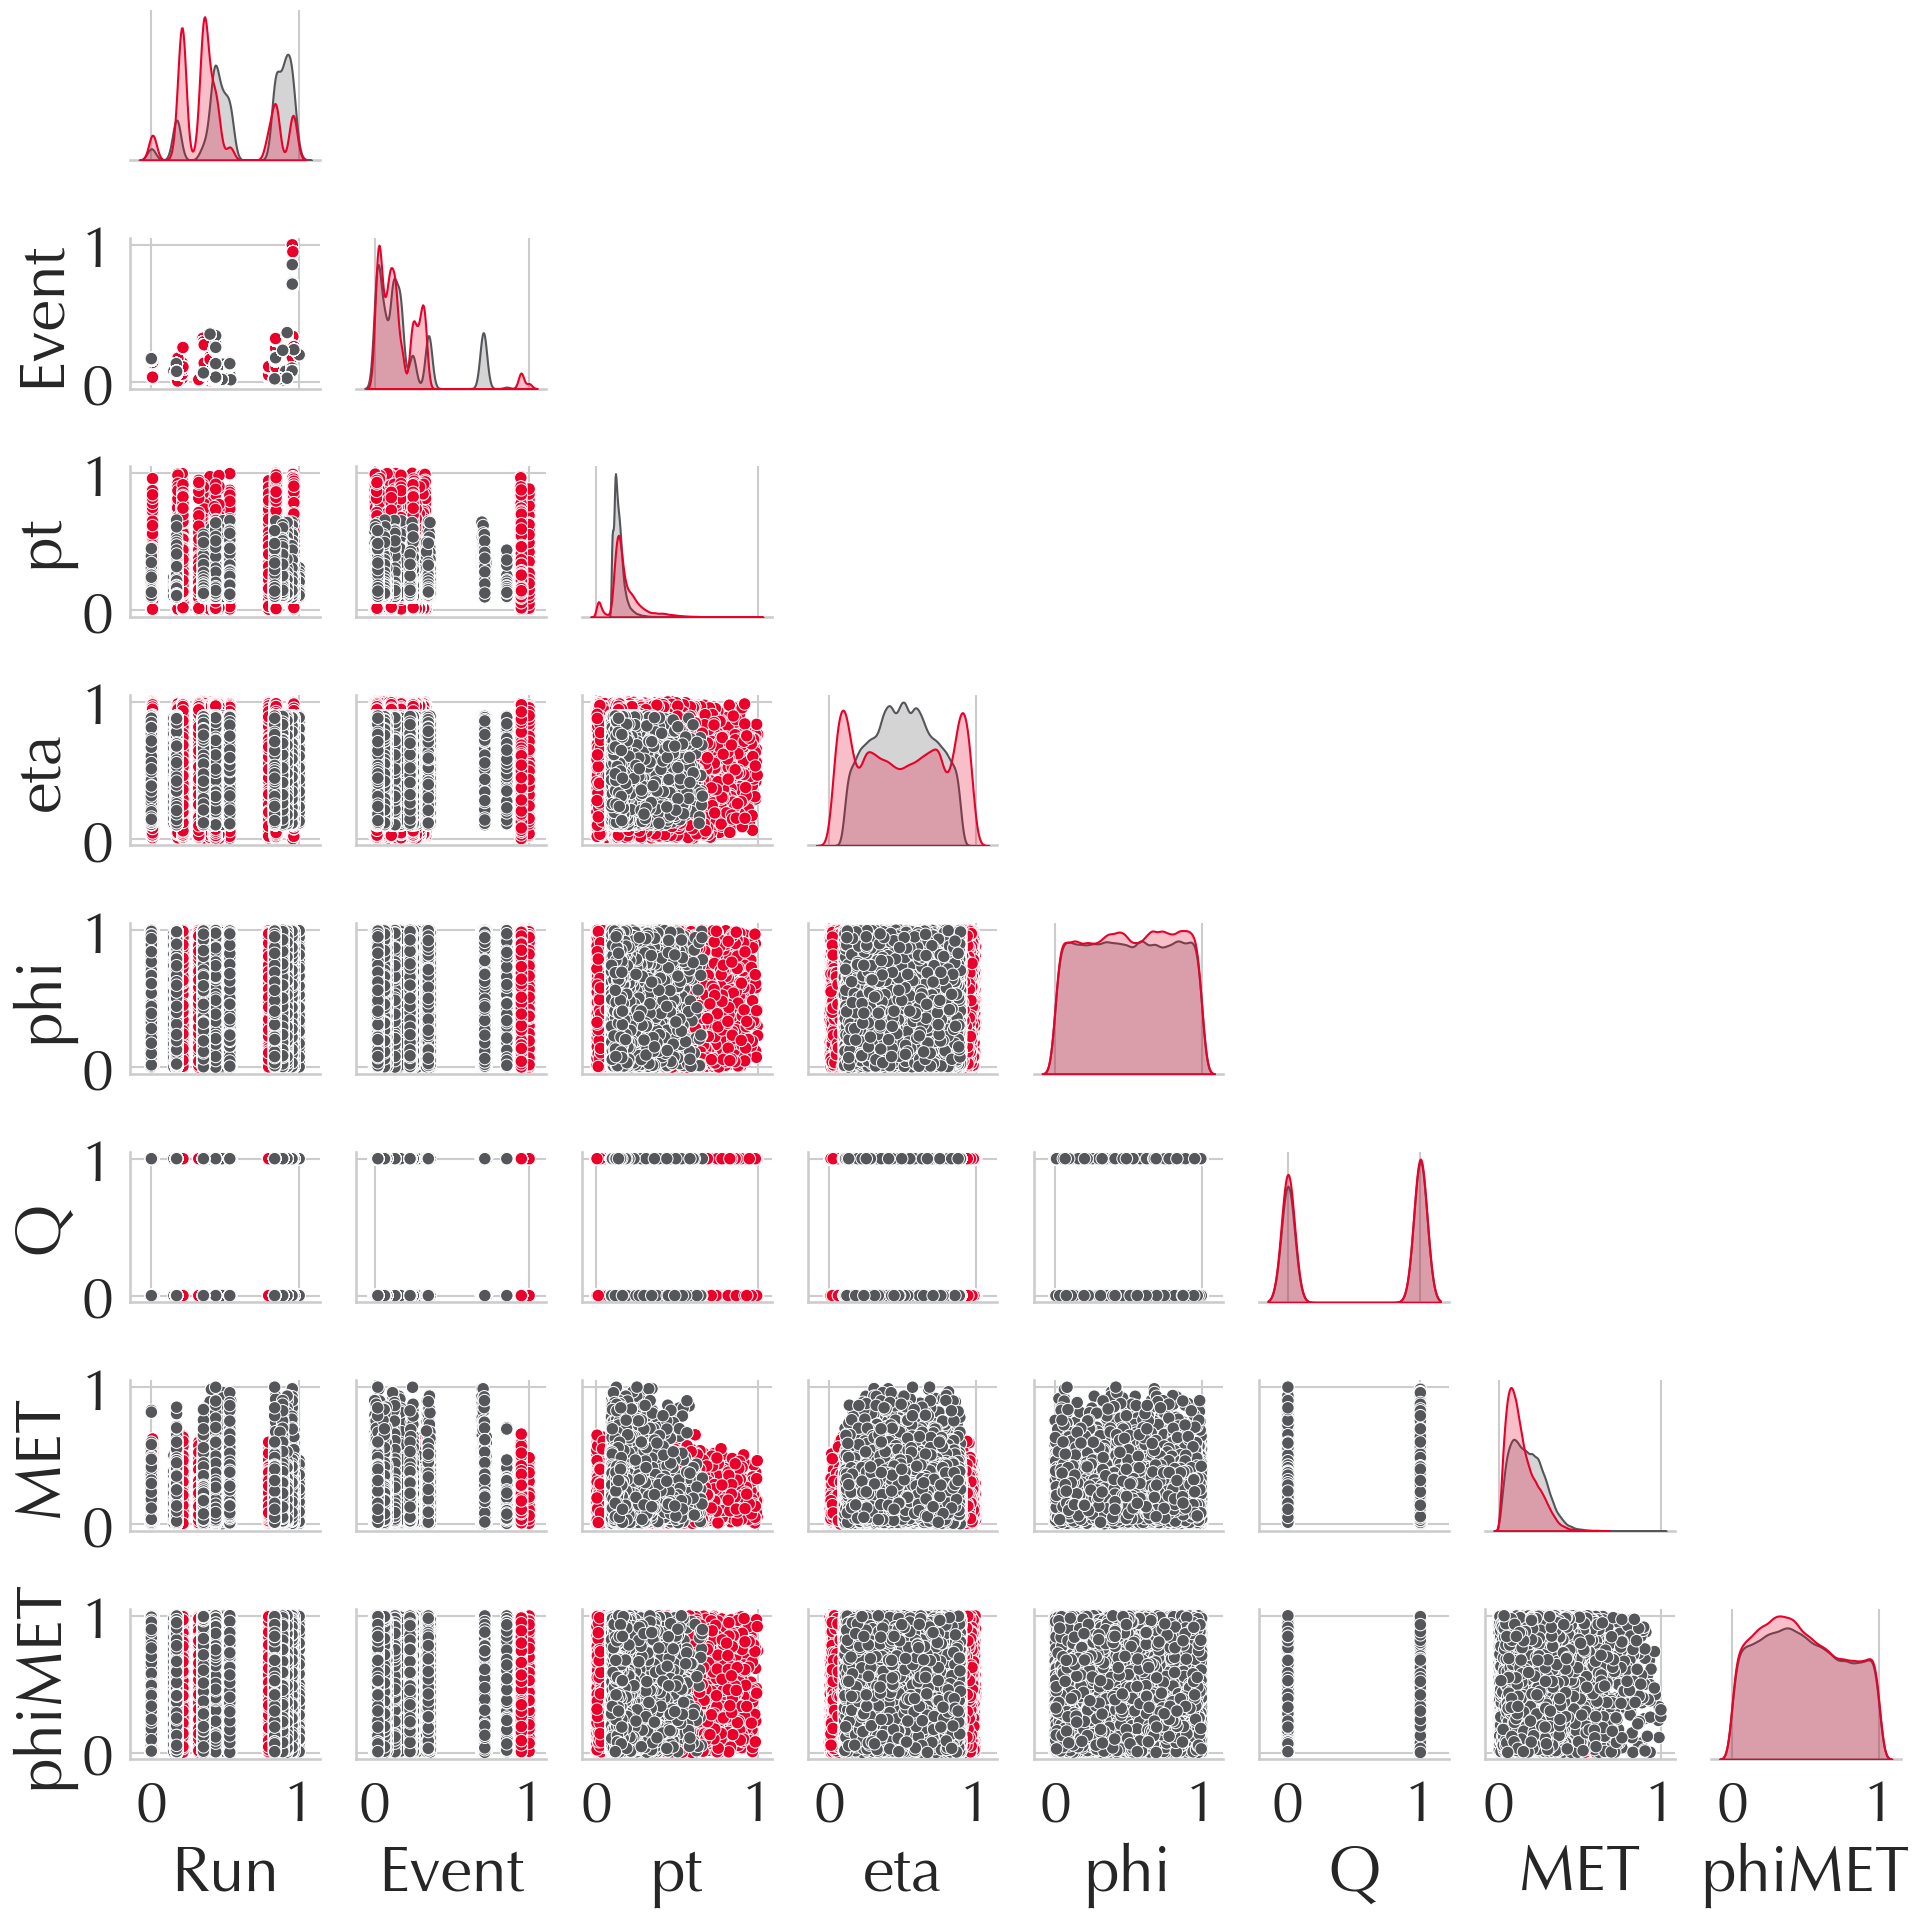
\includegraphics[width=\linewidth]{./Images/Wpairplot_scaled.png}
%   }
    \end{columns}%
  % {\scriptsize
  % Qua voglio dire che ho guardato in faccia i dati (a che scopo? cercare correlazioni evidenti e sbarazzarmi di dati che potrebbero inquinare l'allenamento dla rete), ho rimosso gli outliers e poi li ho riscalati (e dicendo qsto mi collego alla slide successiva pké la ragione dl riscalamento è strettamente legata agli algoritmi)

  % Qua mostriamo sicuramente i pairplot (mi raccomando allora a inserirli riscalati!) che sono la cosa più indicativa   
  % Raccontiamo la storia di correlazioni evidenti che permetterebbero una facile classificazione, nel caso $+$ semplice attraverso 1 appl lineare

  % I concetti da far passare sono 2: è meglio avere 1 dataset uniforme, quindi scaliamo tutto e ci sbarazziamo degli outlier, evitare di introdurre ridondanze (ie guardare in faccia i dati con pairplot)
  % }

  % {\scriptsize
  % la qstione dgli outlier dettagliata in slide di backup con i boxplot -> in questa maniera escono $+$ slides (e qua posso sprecarmi con il logaritmo e lo questione del'approccio scartato con le sigma)
  % }
\end{frame}

\begin{frame}{Suddivisione del dataset}
  \begin{columns}
      \column{.4\linewidth}
      \begin{figure}
        \resizebox{\textwidth}{!}{
          \begin{tikzpicture}
            \coordinate (A) at (0,0);
            \coordinate (B) at (8,0); % this is the width of the rectangle
            \coordinate (C) at (8,10);
            \coordinate (D) at (0,10); % this is the height of the rectangle
            \coordinate (AB) at (6.4,0); % qsto voglio che sia a 0.8 AB
            \coordinate (AD) at (0,2); % qsto voglio che sia a 0.2 AD
            \useasboundingbox (A) rectangle (C);

            \only<1>{
              \draw [unitocolor, fill=unitocolor!70] (A) -- (B) -- (C) -- (D) -- (A);
              \path (4,5.5) node (dataset)[line width=.1cm, text width=5cm] {\begin{center}\huge\bfseries\color{white}Dataset\end{center}};
            }
            \only<2>{
              \draw [unitocolor, fill=unitocolor!70] (A) -- ($(AB) - (1pt,0)$) --++ (D) -- (D) -- (A);
            }
            \only<2->{
              \draw [faircolor, fill=faircolor!80] ($(AB) + (1pt,0)$) -- (B) -- (C) -- ($(AB) + (1pt,0) + (D)$);
            }
            \only<3->{
              \draw [unitocolor, fill=unitocolor!80] ($(AD) + (0,1pt)$) -- ($(AB) + (AD) + (-1pt,1pt)$) --++ ($(D) - (AD) - (0,1pt)$) -- (D) -- ($(AD) + (0,1pt)$);
              \draw [unitograyA, fill=unitograyA!80] (A) -- ($(AB) - (1pt,0)$) --++ ($(AD) - (0,1pt)$) -- ($(AD) - (0,1pt)$) -- (A);
            }
            % sadly the coordinates for text are hard coded :(
            \only<2->{
              \path (7.2,5.9) node (test)[line width=.1cm, text width=.4cm, minimum height=5cm] {\begin{center}\huge\bfseries\color{black}T\linebreak e\linebreak s\linebreak t\end{center}};
            }
            \only<3->{
              \path (3.2,1.4) node (val)[line width=.1cm, text width=4cm] {\begin{center}\huge\bfseries\color{white}Validation\end{center}};
              \path (3.2,6.2) node (train)[line width=.1cm, text width=3cm] {\begin{center}\huge\bfseries\color{white}Train\end{center}};
            }
          \end{tikzpicture}
        }
      \end{figure}
      \vspace*{1.5ex}

    \column{.55\linewidth}
      Bisogna evitare di insegnare alla rete il rumore statistico dei dati
      \begin{itemize}
        \item<2->Test: per verificare che la rete generalizzi
        \item<3->Train: per allenare la rete
        \item<3->Validation: per valutare l'allenamento della rete
      \end{itemize}


    \end{columns}
    % e qua il collegamento con la slide successiva viene facilissimo
\end{frame}

\section{Reti Neurali}
\subsection{Architettura e principi}
\begin{frame}
  \centering
  \Huge\bfseries
  Reti Neurali
\end{frame}

\begin{frame}{L'architettura}
  \vspace*{4.5ex}
  \begin{figure}
    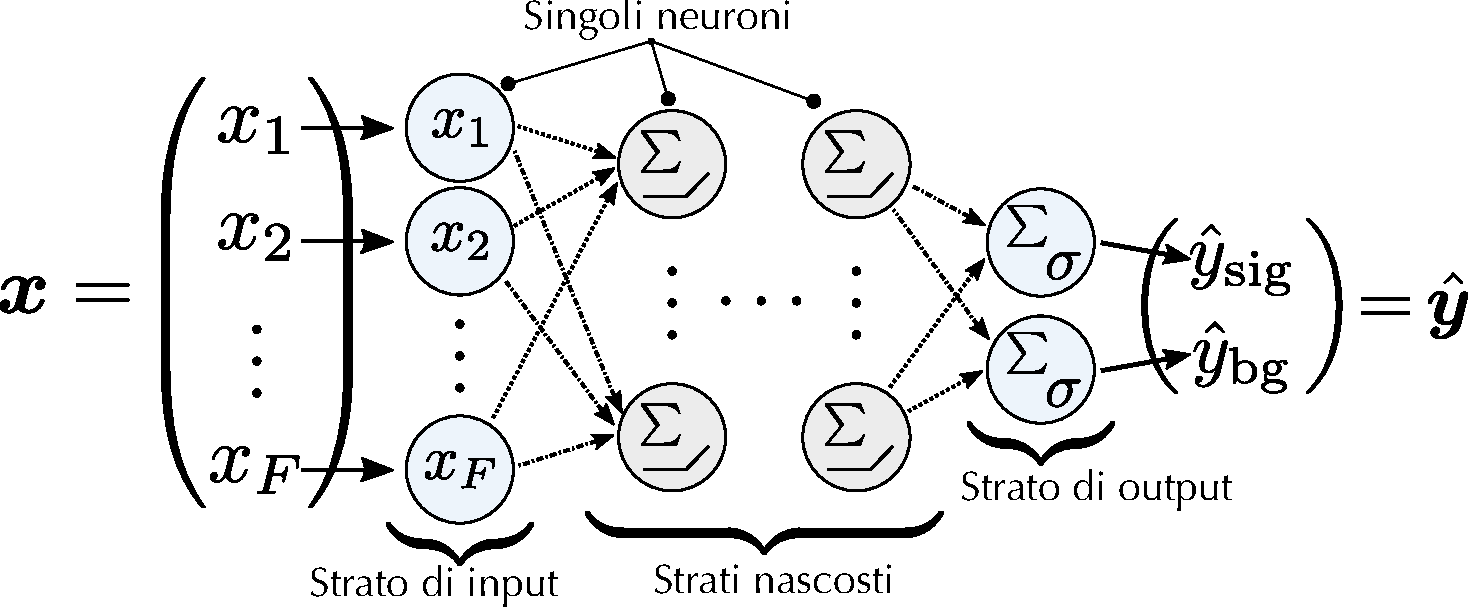
\includegraphics[width=\linewidth]{./Images/fcn-architecture-simple-flat.pdf}
  \end{figure}
  \begin{flushright}
    \vspace*{2.0ex}
    \scalebox{.4}{\color{unitograyA!65}
      Adapted from: https://github.com/ejmastnak/fmf-seminar/blob/main/media/vector/fcn-architecture-simple.pdf
    }
  \end{flushright}
% Qua bisogna introdurre i parametri su cui ho agito: numero di layer, nodi, attivazione, algoritmo di ottimizzazione (questo nella slide successiva)
% ricordati di specificare quand'è che la rete prende il nome di 'deep'
% E devo spiegare come funziona la questione dei parametri (pesi e bias) e dove si introduce la non linearità (attivazione)
\end{frame}

\begin{frame}{Loss function \\Algoritmi di ottimizzazione}
  \vspace*{-4ex}
  \begin{multline*}
    P(\mathcal{D}|\bm{w}) = \prod_{i=1}^{n} q(x_i|\bm{w})^{p(x_i)}\, \qty(1-q(x_i|\bm{w}))^{1-p(x_i)}\\[-2ex] {\color{unitocolor}\leadsto}\quad H(p,q) = - \sum_{i=1}^{n} p(x) \log q(x)
  \end{multline*}
% che è la massima verosimiglianza del dataset osservato (di cui si studia e minimizza la - log likelyhood)
  \begin{columns}[T]
    \column{.6\linewidth}
      \vspace*{-6ex}
      \begin{figure}
        \centering
%       \begin{tikzpicture}
%         \node [draw, line width=.04cm, inner sep=0pt, text width=\linewidth, minimum height=5cm] (landscape) at (0,0) {
%           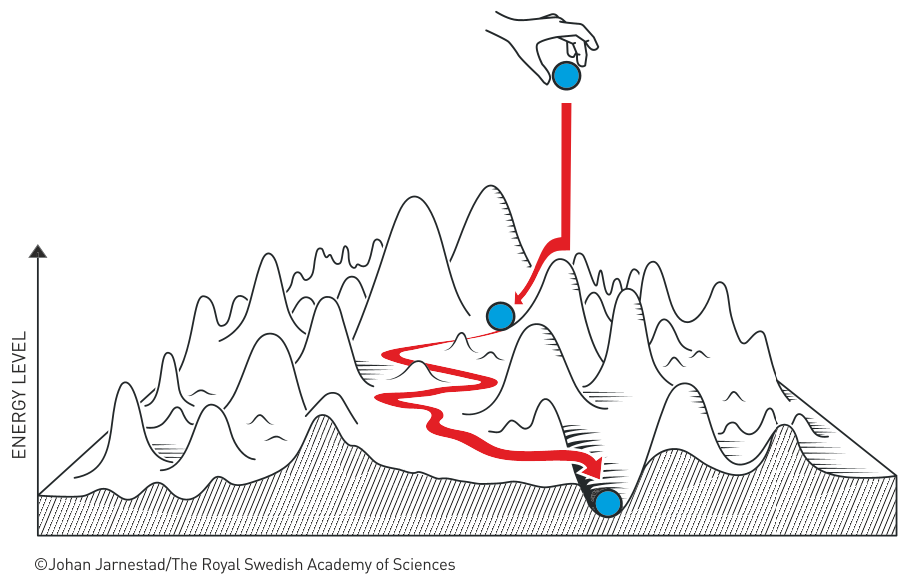
\includegraphics[width=\textwidth]{./Images/loss_landscape.pdf}
%         };
%         \node [draw, line width=.04cm, anchor=west, inner sep=0pt, text width=5cm] (loss) at ($(landscape) + (-3,3.3)$) {
%           \begin{equation*}
%             H(p,q) = - \sum p(x) \log q(x)
%           \end{equation*}
%         };
%       \end{tikzpicture}
        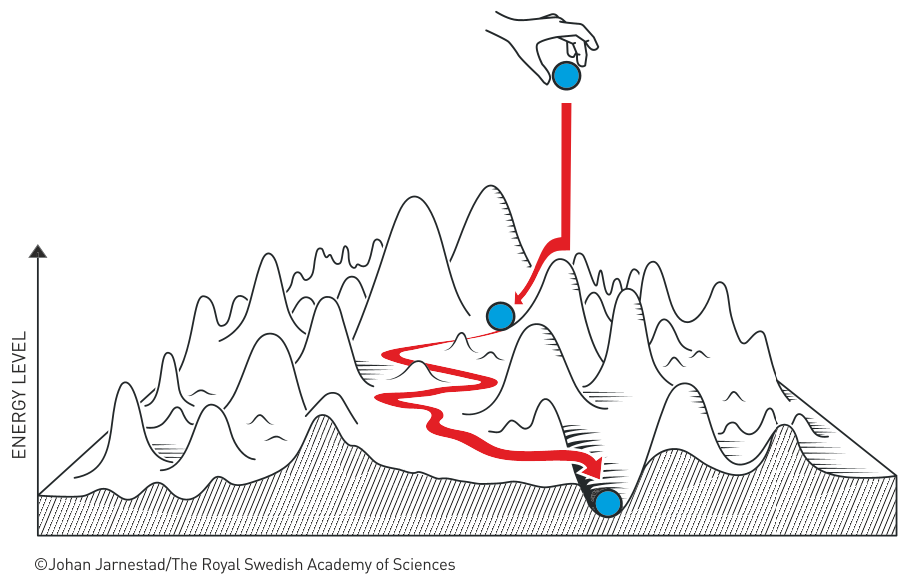
\includegraphics[width=\textwidth]{./Images/loss_landscape.pdf}
      \end{figure}
    \column{.35\linewidth}
      \vspace*{.5ex}
    % \begin{equation*}
    %   H(p,q) = - \sum p(x) \log q(x)
    % \end{equation*}
      \begin{itemize}
        \item Gradient Descent
        \item RMS
        \item Adam
        \item Nadam
        \item \dots
      \end{itemize}
  \end{columns}

  % Qsto per spiegare come funzioni la rete, nn per mostrare risultati ancora
% L'idea di 1 loss function da minimizzare (come se fosse un'energia), qsta nn è semplice da spiegare visivamente, di questa metterei proprio la formula così la commento un attimo
%
% Algoritmo (sarebbe carino accennare al learning rate e al momento e all'adattività degli algoritmi)
%
%
% Immagini di allenamenti significativi, magari anche in cui si veda l'overfitting
\end{frame}

\begin{frame}{Overfitting}
  \vspace*{3.5ex}
  \begin{columns}
    \column{.48\linewidth}
      \centering
      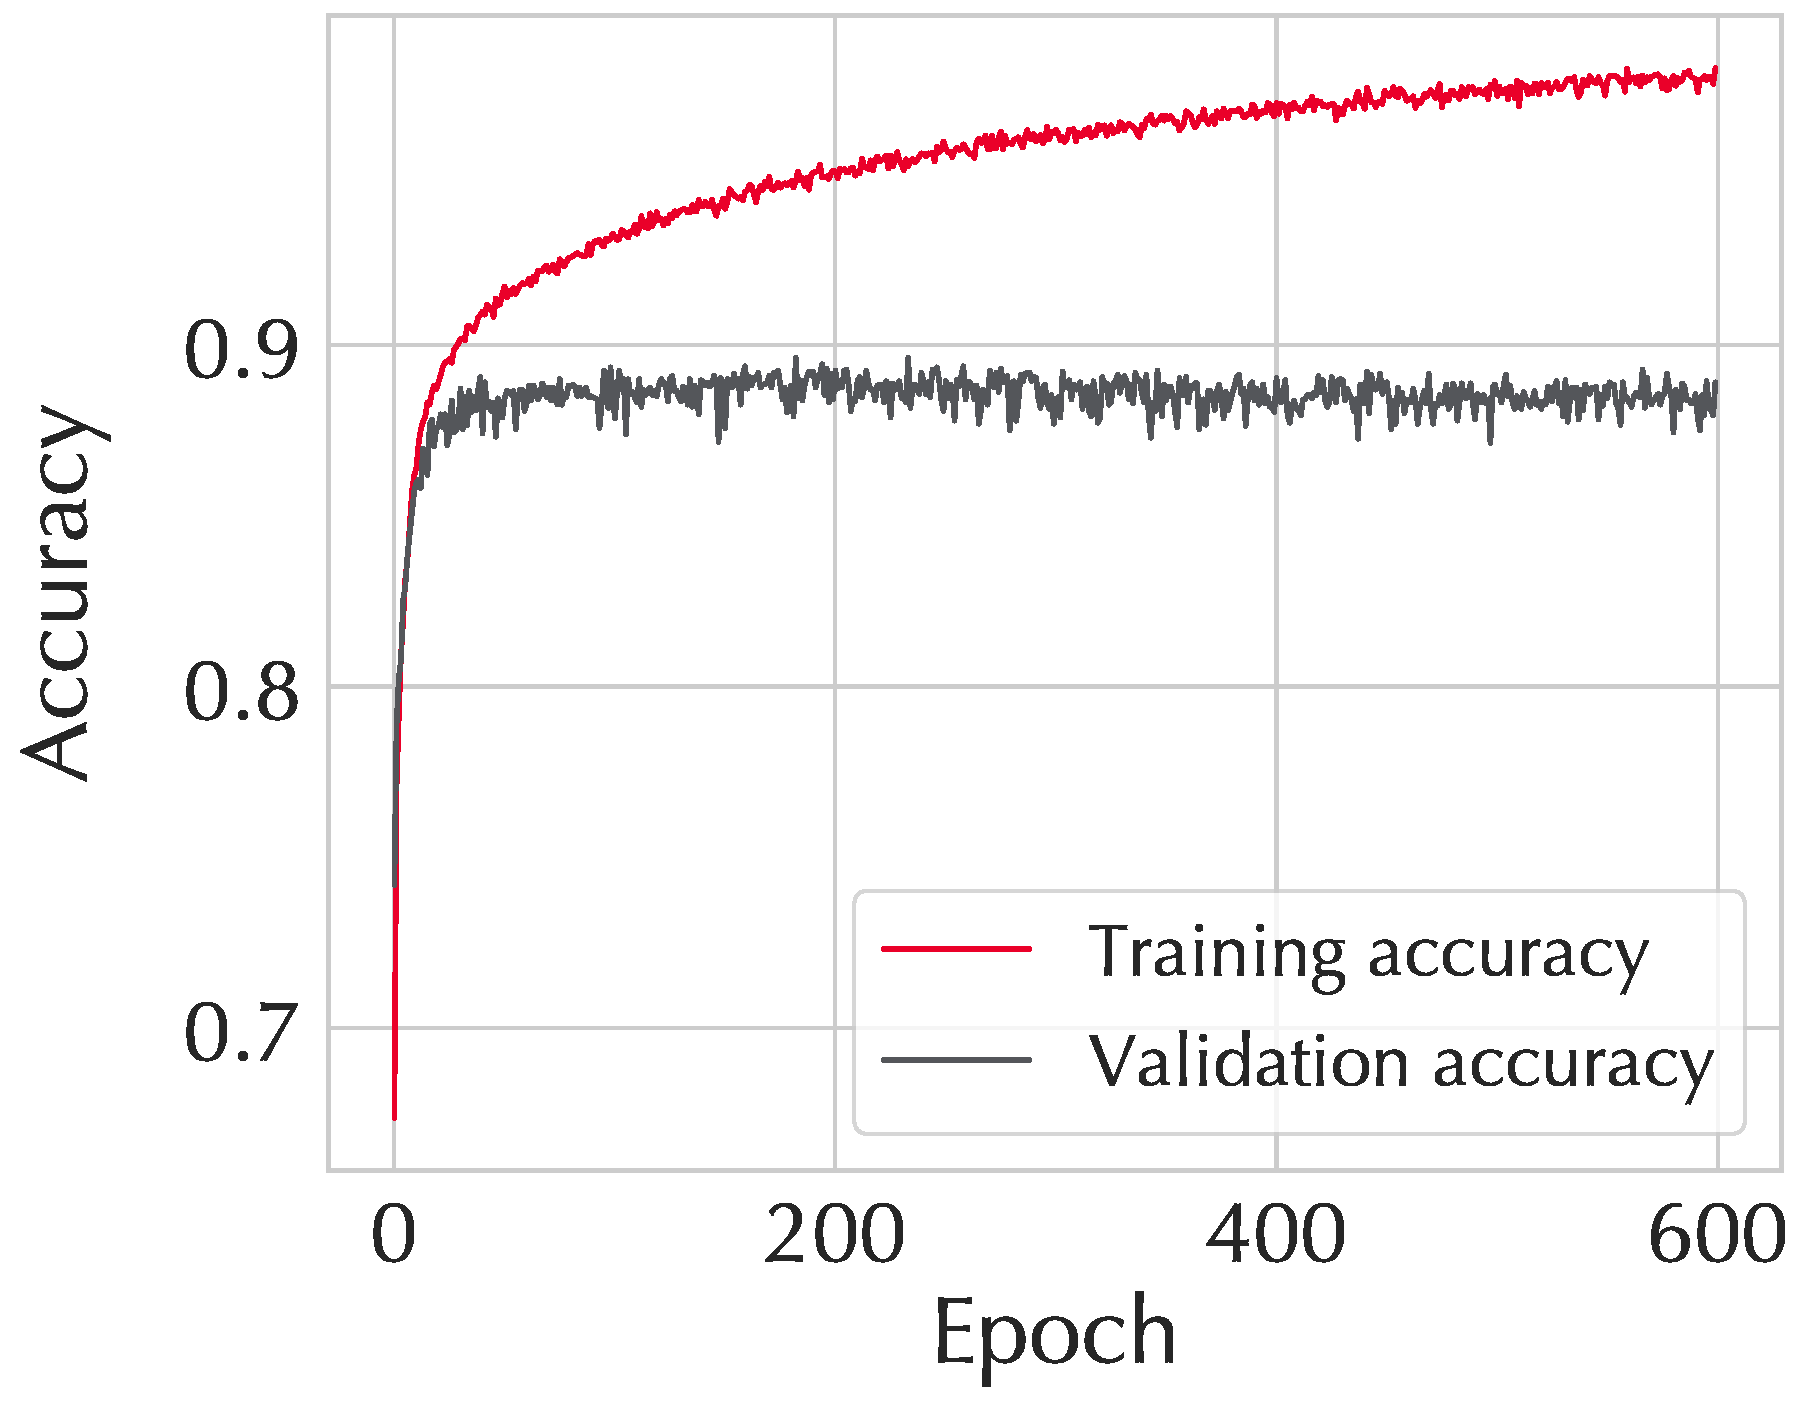
\includegraphics[width=\linewidth]{./Images/Z64_64_adam_relu_acc.pdf}
    \column{.48\linewidth}
      \centering
      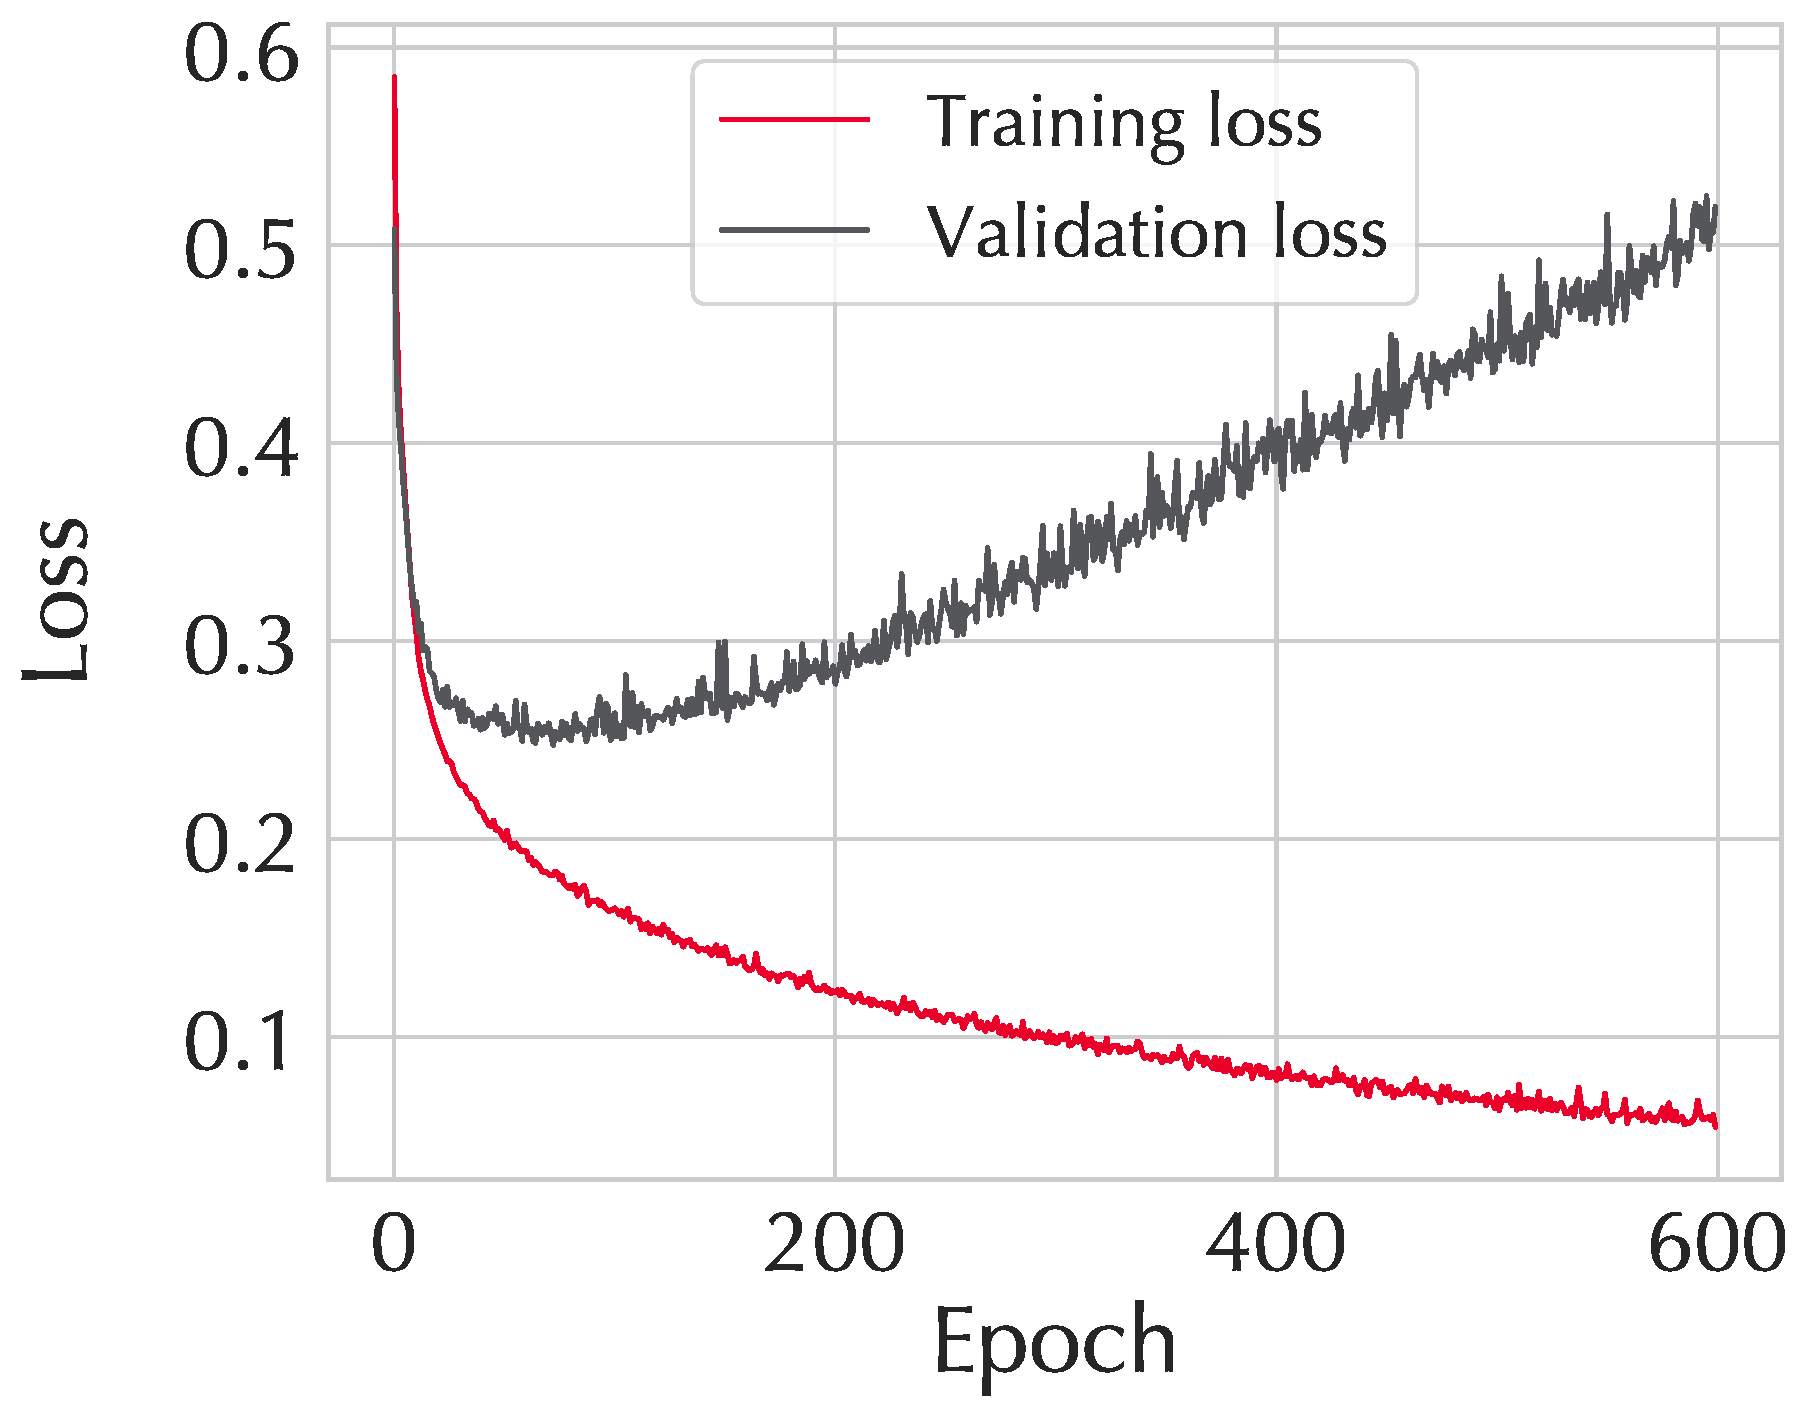
\includegraphics[width=\linewidth]{./Images/Z64_64_adam_relu_rock.pdf}
  \end{columns}
\end{frame}


\section{Risultati}
\begin{frame}
  \centering
  \Huge\bfseries
  Risultati
\end{frame}

\begin{frame}{Risultati - Dataset \only<1-2>{$Z$}\only<3->{$W$}}
  \vspace*{2.5ex}%
  \only<1-2>{architettura: \parbox{12ex}{(64,64)} algoritmo: Adam\qquad attivazione: sigmoide}%
  \only<3>{architettura: \parbox{12ex}{(6,6)} algoritmo: Adam\qquad attivazione: relu}%
  \only<4>{architettura: \parbox{12ex}{(24,12,24)} algoritmo: Adam\qquad attivazione: sigmoide}%
  \vspace*{2.0ex}
  \parbox[c][.4\textwidth]{\textwidth}{
    \begin{columns}
      \column{.45\linewidth}
        \centering
        \only<1-2>{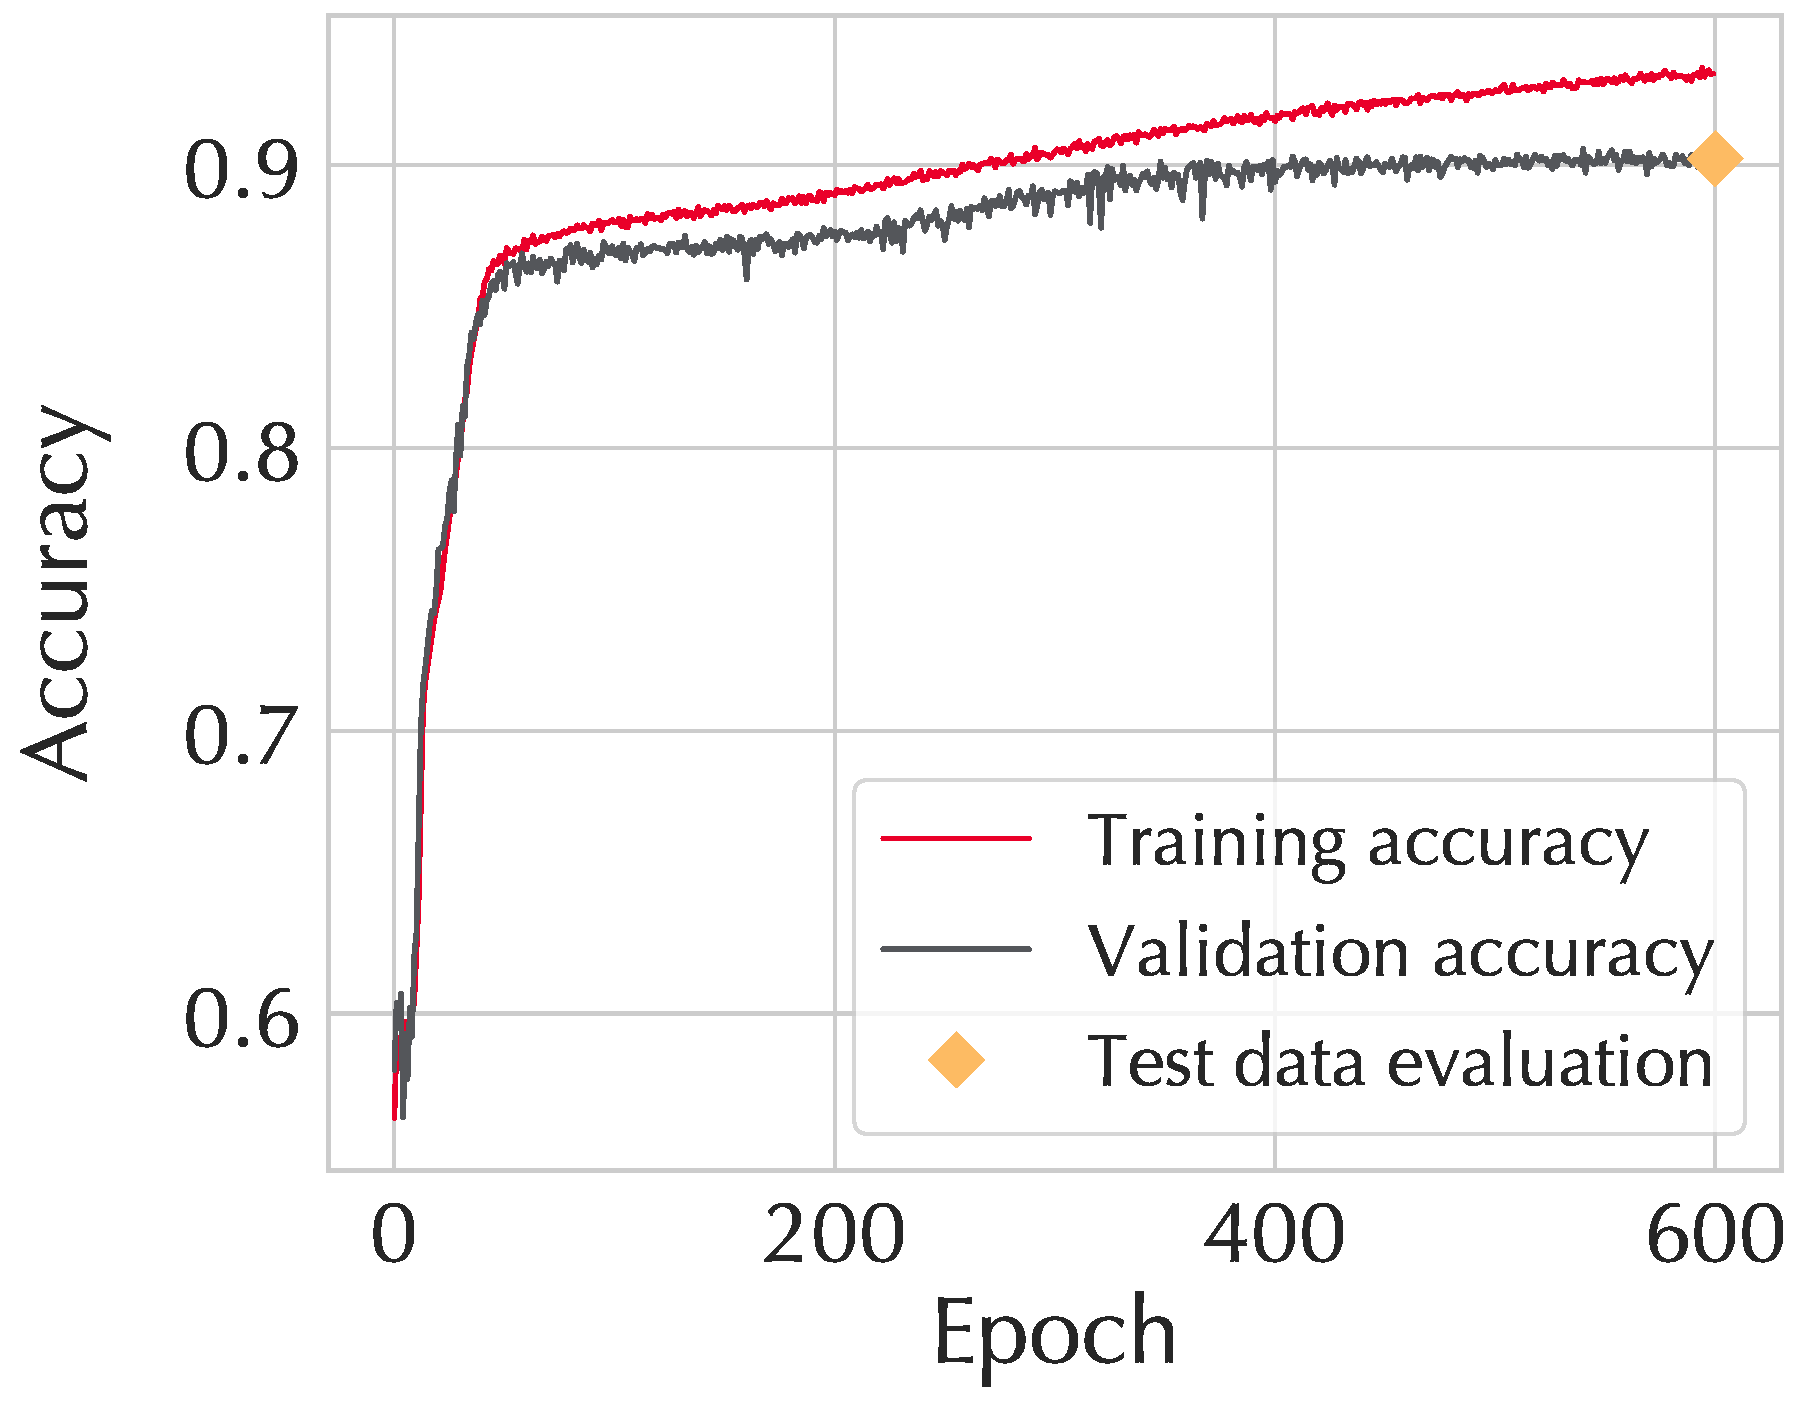
\includegraphics[width=\linewidth]{./Images/Z64_64_adam_sigmoid_acc.pdf}}
        \only<3>{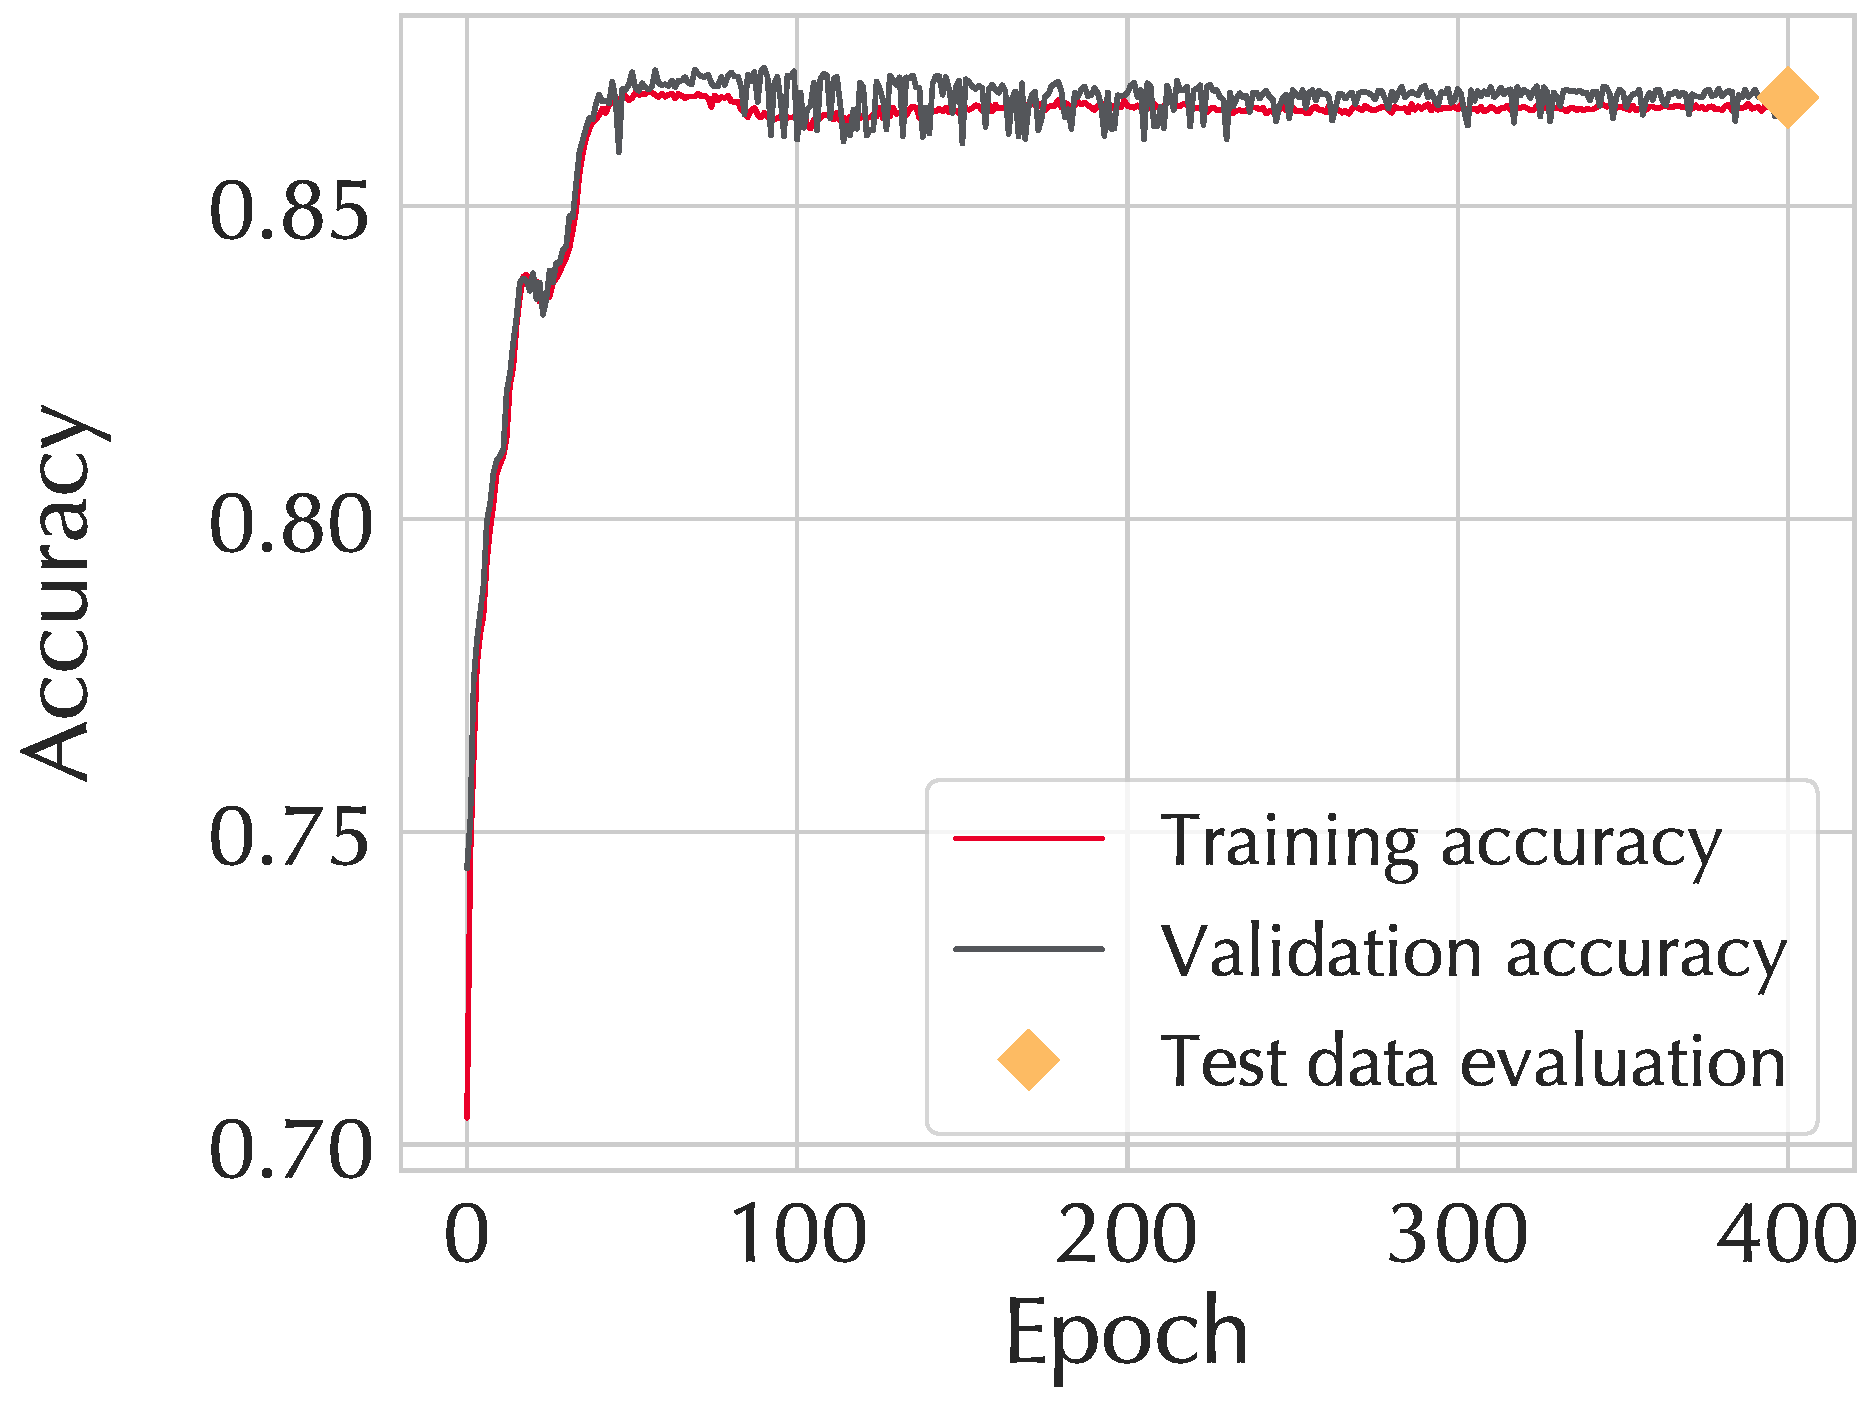
\includegraphics[width=\linewidth]{./Images/W6_6_Adam_relu_acc.pdf}}
        \only<4>{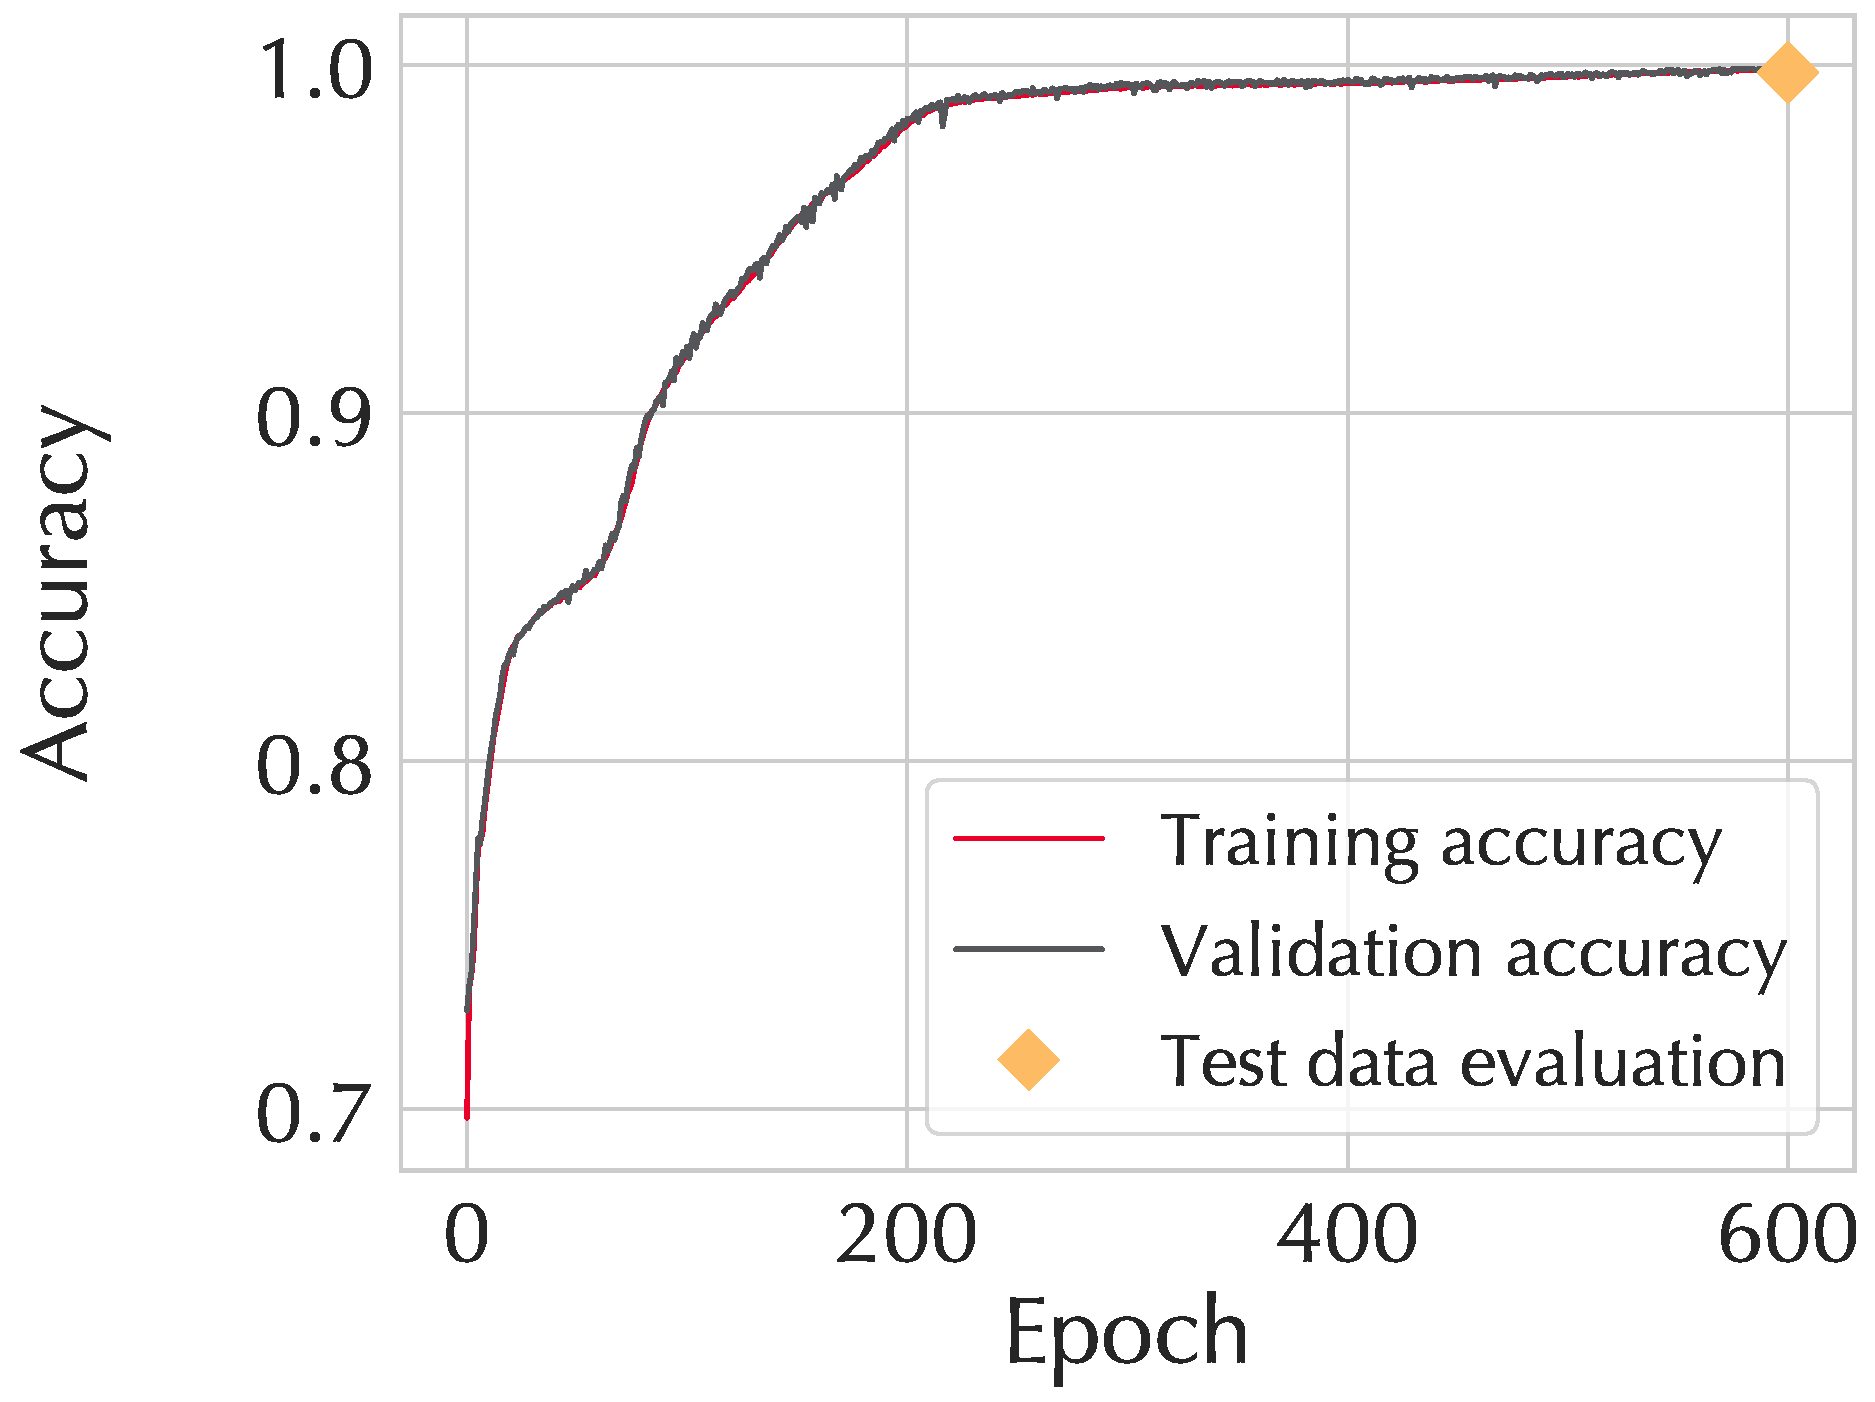
\includegraphics[width=\linewidth]{./Images/W24_12_24_Adam_sigmoid_acc.pdf}}
      \column{.45\linewidth}
        \centering
        \only<1-2>{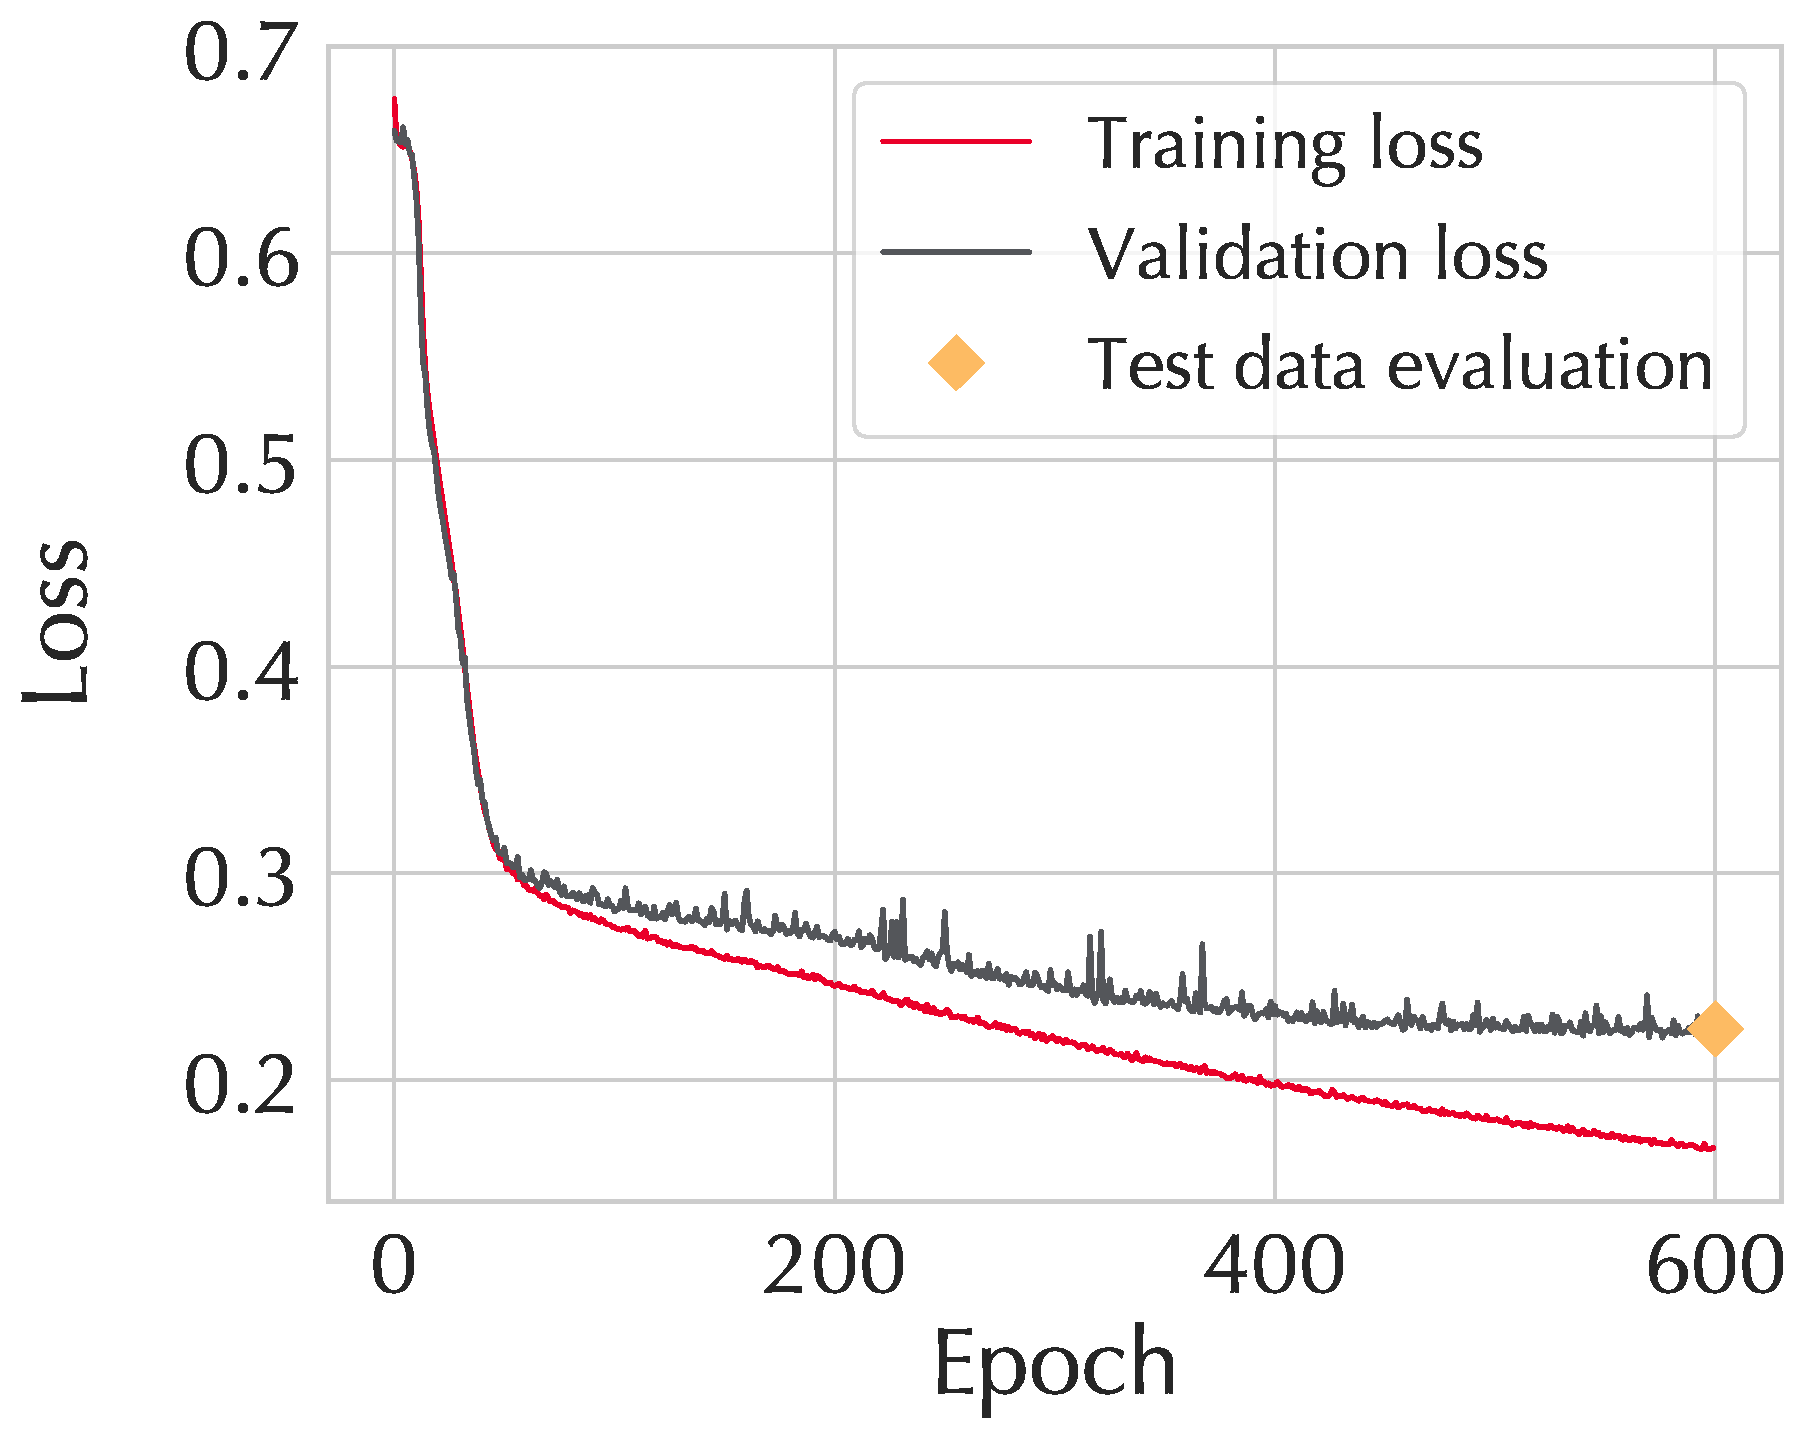
\includegraphics[width=\linewidth]{./Images/Z64_64_adam_sigmoid_rock.pdf}}
        \only<3>{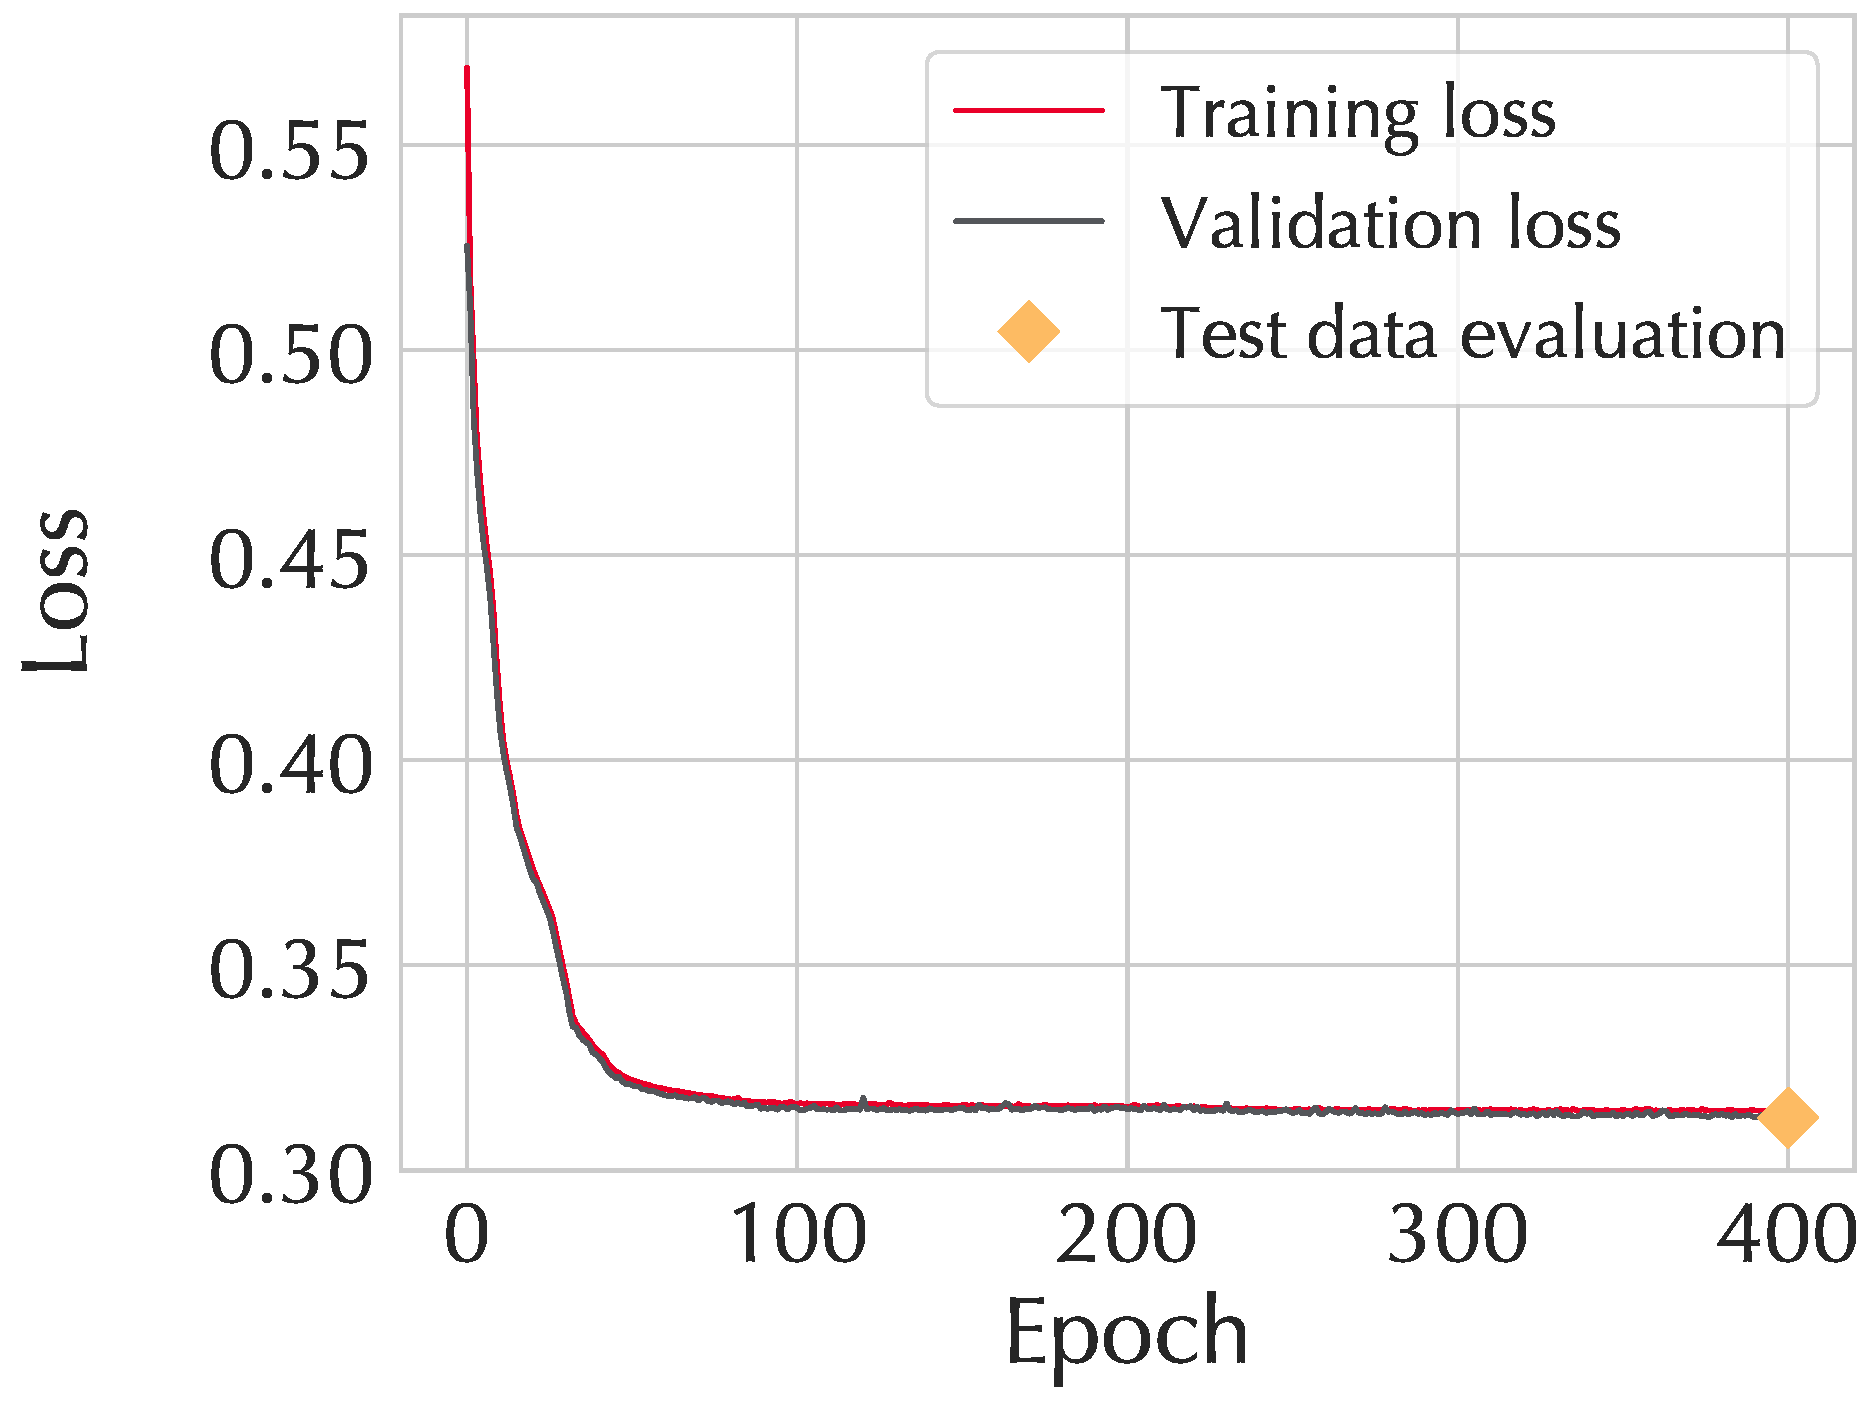
\includegraphics[width=\linewidth]{./Images/W6_6_Adam_relu_rock.pdf}}
        \only<4>{\includegraphics[width=\linewidth]{./Images/W24_12_24_adam_sigmoid_rock.pdf}}
    \end{columns}%
  }%
  \vspace*{-.5ex}
  \only<1>{\color{white}}Il modello generalizza al test set
  \vspace*{.2ex}
  \begin{center}
    \scalebox{.8}{
      $\color{unitocolor!60}\boldsymbol{\big[}$
      {\scriptsize\color{unitograyA!65}
        https://github.com/jlancione/thesis\_notebooks
      }%
    }%
    $\color{unitocolor!60}\bm{\big ]}$
  \end{center}
\end{frame}


\section{Conclusioni}
\begin{frame}
  \centering
  \Huge\bfseries
  Conclusioni
\end{frame}

\begin{frame}{Conclusioni}
  \begin{itemize}
    \item Le reti neurali si prestano molto bene all'identificazione di particelle
    \item L'allenamento è efficace perché \textbf{generalizza} al test set
    \item Ho identificato una classe di \textbf{modelli equivalenti}
  \end{itemize}
  \vspace{2ex}

  Ulteriori sviluppi: 
  \begin{itemize}
    \item Combinare i dataset rimuovendo le labels per allenare una rete a distinguere i bosoni tra loro
    \item Utilizzare una di queste reti come modello generativo per simulare decadimenti
    % anche con parametri #i! ie (ESTRAPOLARE! in tutte le sue accezioni e applicazioni) a energie maggiori/ al di fuori dl'accettanza dl rivelatore in vista di futuri rivelatori (ie può essere interessante andare a guardare lì?)
  \end{itemize}
%
%   \vspace*{2ex}
  \begin{columns}
    \column{.25\linewidth}
    {
      \only<1>{\setbeamercolor{block body}{bg=white, fg=white}}
      \only<2>{}
      \begin{block}{}
        \centering\vspace*{.5ex}
        \Large\bfseries
        \color{white}
        Grazie%
        \vspace*{.8ex}
      \end{block}
    }
  \end{columns}
\end{frame}

\end{document}
